% = = = = = = = = = = = = = = = = = = = = = = = = = = = = = = = = = = = = = = = = = = = = =
% P  R  E  A  M  B  L  E
% = = = = = = = = = = = = = = = = = = = = = = = = = = = = = = = = = = = = = = = = = = = = =
\documentclass[12pt]{article}
\usepackage{amsmath, amssymb, authblk}
%\usepackage{array}
\usepackage{booktabs}
\usepackage{bm}
\usepackage[small,labelfont=bf,up,singlelinecheck=false]{caption}
%\usepackage{fancyhdr}
%\usepackage[T1]{fontenc}
\usepackage[bottom]{footmisc}
\usepackage{geometry}
\usepackage{graphicx}
\usepackage{hyperref}
%\usepackage[utf8]{inputenc}
	%\inputencoding{latin1}
	%\inputencoding{utf8}
%\usepackage{lettrine}
%\usepackage[sc]{mathpazo}
%\usepackage{lmodern} % Nice fonts?
%\usepackage{mathrsfs}
\usepackage{mathtools} 
\usepackage{marvosym} % silly bullet-point symbols (misc symbols)
%\usepackage{microtype}
\usepackage{minitoc}         % left in case it is needed elsewhere
\setcounter{secttocdepth}{5} % idem
\usepackage{etoc} % for toc before each section.a
%\usepackage{multicol}
\usepackage{needspace}
\usepackage{paralist}
%\usepackage{polynom} 			% typesetting polynomial long division
%\usepackage{setspace}
%	\onehalfspacing 
\usepackage[compact]{titlesec} 		% compact shrinks whitespace around section headings.
% \usepackage{ulem} 				% for strikeout \sout command.
%\usepackage{verbatim}

% Muh packagez :)
\usepackage{../Packages/MathCommands}
\usepackage{../Packages/BrandonColors}
\usepackage{../Packages/BrandonBoxes}
\usepackage{../Packages/NoteTaker}
\usepackage{../Packages/MachineLearningUtils}

\newcommand\myfig[2][0.3\textwidth]{\begin{figure}[h!]\centering\includegraphics[width=#1]{#2}\end{figure}}
\newcommand{\myspace}{\vspace{2\bigskipamount}}
\newcommand\p{\Needspace{10\baselineskip} \noindent}
\newcommand\Var[1]{\text{Var}\left[#1\right]}

\usepackage{layout} % Type \layout() anywhere to see values of layout frame.
%\usepackage{showframe} % Displays layout frame on all pages
\usepackage{marginnote}
\renewcommand*{\marginfont}{\scriptsize}

\titleformat*{\subsubsection}{\large\scshape}

\newcommand{\y}{\vec y}

% Title
\title{\vspace{-10mm}\fontsize{24pt}{8pt}\selectfont\textbf{Fall 2016 Course Notes}\vspace*{-4mm}}
% Author
\author{Brandon McKinzie}
% Date
\date{}

% --------------------------------------------------------------
% --------------------------------------------------------------

\renewcommand{\matr}[1]{\mathbf{#1}}

\begin{document}
\dosecttoc
\tableofcontents
%\fontsize{10}{10.2}
%\selectfont


\mysection{Machine Learning \\ CS 189}\label{Machine Learning}
\lecture{Machine Learning}{Classification}{August 30}

\p \blue{Goal:} Want to prove that $w$ is normal to decision boundary.
\begin{itemize}
	\item Starting axiom: Any vector $x$ along the decision boundary satisfies, by definition,
	\begin{equation}
		w \cdot x + \beta = 0
	\end{equation}
	\item Let $x$ and $x'$ be two such vectors that lie on the decision boundary. Then the vector $x' - x$ points from $x$ to $x'$ and is parallel to the decision boundary. If $w$ really is normal to the decision boundary line, then
	\begin{align}
	\begin{split}
	w \cdot (x' - x) &= 0 \\
	&= w \cdot x' - w \cdot x \\
	&= (w \cdot x' + \beta) - (w \cdot x + \beta) \\
	&= 0 + 0
	\end{split}
	\end{align}
\item Euclidean distance of $x$ to decision boundary:
\begin{equation}
\tau = - \frac{(w \cdot x + \beta)}{||w||} = - \frac{f(x)}{||w||}
\end{equation}
\item The \blue{margin} is can be found as the minimum over all training data $\tau$:
\begin{equation}
M = \min_{i \in 1 \cdots n} \frac{|f(x_i)|}{||w||}
\end{equation}
\end{itemize}

% ==================================================================
%===================================================================
% 09/01 STOCHASTIC GRADIENT DESCENT
% ==================================================================
% ==================================================================
\lecture{Machine Learning}{Gradient Descent}{September 1}

\begin{itemize}
	\item \blue{Optimization:} maximize goals/minimize cost, subject to constraints. However, can model a lot while ignoring constraints.
	\item Main optimization algorithm is \blue{stochastic gradient descent}.
	\item The \red{SVM}\footnote{so-called because you could represent the decision boundary as a set of vectors pointing to the hyperplane.} is just another cost function. Want to minimize\footnote{Notation: $(z)_+ = max(z, 0)$.}
	\begin{equation}
	C \displaystyle\sum_{i=1}^{n} \big(1 - y_i ( w \cdot x_i + \beta) \big)_+ + ||w||^2
	\end{equation}
	with respect to the \blue{decision variables} $(w, \beta)$; Note that $C$ is a \blue{hyperparameter}.
\end{itemize}

%


% ==================================================================
% ==================================================================
\lecture{Machine Learning}{Stochastic Gradient Descent}{September 6}

\begin{itemize}
	\item Review: minimize cost function $f(w)$ over w. Take gradient; set to zero to solve for $w$.
	\item If can't solve analytically, then Gradient Descent:
		\begin{equation}
		w_{k+1}= w_k - \alpha_k \nabla f(w_k)
		\end{equation}
	\item For convex $f$, can always find solution. Guaranteed global minimum.
	\item Cost functions of form: $\text{minimize }\sum \text{loss}(w_i(x_i, y_i)) + \text{penalty }(w)$.
	\item SVM example: \[\text{min } C/n \sum (1 - y_i w^T x_i)_+ + ||w||^2 \]. Add squared norm because better margins and better classifications. Also, because algorithms converge faster. C is the \blue{regularization parameter}. ``Do I fit the data, or make w simple?''. Doesn't change optimal set, just changes the ``Cost'' (wat).
	\item Want algorithm constant in number of data points $n$\footnote{Regular GD is linear in $n$}.
	\item Unbiased estimate of the gradient:
	\begin{itemize}
		\item Want  vlaue of $g$ to be gradient of cost function.
		\item Sample $i$ uniformly at random from $\{1, \ldots, n\}$.
		\item Then set $g$ to gradient of loss at ith data point.
	\end{itemize}
	\item SGD:
	\begin{itemize}
		\item initialize $w_0$, $k$ = 0.
		\item (Repeat) sample $i$ at uniform. Do weight update on the loss for $i$ term. Until converged.
		\item Follow the  value of the gradient (rather than the true gradient) until converge. Following a noisy version. As long as variance is bounded, direction will be more or less correct. For large number of data points $n$, will be pretty good.
	\end{itemize}
	\item Numerical example:
	\begin{itemize}
		\item $f(w) = 1/2n \sum (w - y_i)^2$. Assumes x always 1.
		\item Solve $\nabla f(w) = 0 = 1/n \sum (w - y_i) = 0$.
		\item Optimal $w = 1/n \sum y_i $. The empirical mean.
		\item Init $w_1 = 0$. Set $\alpha_k = 1/k$. Where $k$ is $kth$ update reference.
		\item $w_2 = w_1 - \alpha_k \nabla \text{loss }() = y_1$. Where loss the grad of f.
		\item $w_3 = w_2 - \alpha_2 (w_2 - y_2) = y_1 -\frac{1}{2}(y_1 - y_2) = \frac{y_1 + y_2}{2}$.
		\item $w_4 = \cdots = $. idk
		\item Lesson: order we passed through data didn't matter. One pass over all data points leads to optimal $w$. Why advocate randomness then? He uses sum of trig function example to illustrate how SGD can struggle if done in order, but converge much quicker when randomly sampled.
	\end{itemize}
	\item Illustrates "\purple{region of confusion}". Coined by Bertsekas. Different convex functions along w. Rapid decrease in error early on iterations means we are far outside this region. Constant $\alpha$ means you'll jiggle around later iterations. That is why you do diminishing $\alpha$; helps in region of confusion.
	\item Most important rules of SGD: (buzzwords)
	\begin{itemize}
		\item shuffle! Can speed up by as much as 20x.
		\item diminishing stepsize ($\alpha$ learning rate decay). After $n$ steps, set $\alpha = \beta \cdot \alpha$.
		\item \blue{momentum}. $w_{k+1} = w_k - \alpha \nabla l_i(w_k) + \beta_k (w_k - w_{k-1})$. Momentum is in final term. Typical value is 0.9.
	\end{itemize}
	\item Notation: $e(z) = (z < 1)$. Evaluates to 1 or 0.
\end{itemize}

% ==================================================================
% ==================================================================
\lecture{Machine Learning}{Risk Minimization \& Optimization Abstractions}{September 8}
\begin{itemize}
	\item Where do these optimization problems come from?
	\begin{itemize}
		\item General framework: minimizing an average loss + $\lambda$ penalty.
		\item Loss: measures data fidelity.
		\item Penalty: Controls model complexity.
		\item Features/representation: How to write $(x_i, y_i)$.
		\item Algorithms: $\nabla$ cost(w) = 0.
		\item \blue{Risk}: Integral of loss over probability(x, y).
		\item Empirical risk: Sample average. Converges to true Risk with more points; variance decreases.
	\end{itemize}
	\item Begins discussion of splitting up data.
	\begin{itemize}
		\item Let some large portion be the \blue{Training set} and the small remaining data points be the \blue{Validation set}.
		\begin{align}
		R_T &= \frac{1}{n_T} \sum_{train} loss(w, (x_i, y_i)) \\
		R_V  &= \frac{1}{n_V} \sum_{val} loss(w, (x_i, y_i))
		\end{align}
		\item By law of large numbers, can say the $R_V$ will go like $\frac{1}{n_V}$. Looking lots of times at validation set becomes a problem with $n_V \approx 10^4$.
	\end{itemize}
	\item Classification example:
	\begin{itemize}
		\item \purple{Hinge} loss: $(1 - y w^Tx)_+$. Means you're solving a SVM.
		\item Least-Squares:  $(1 - y w^Tx)^2$. Bayes classifiers.
		\item In practice, hinge and LS perform basically the same.
		\item Logistic loss useful for MLE.
	\end{itemize}
	\item Most important theorem in machine learning: Relates risk with empirical risk:
	\begin{align}
	R[w] &=  \frac{R[w] - R_T[w]}{\text{generalization err}} + \frac{R_T[w]}{\text{train err}} \\
	&\approx R_V[w] - R_T[w] + R_T[w]
	\end{align}
	\item One vs. all classifation MNIST example: Have a classifier for each digit that treats as (their digit) vs. (everything else). Choose classifier with highest margin when classifying digit.
	\item \blue{Maximum Likelihood}:
	\begin{itemize}
		\item Have $p(x,y; w)$. Pick the $w$ that makes data set have highest probability.
		\item Assumes data points come independently.
		\item Can get same result by minimizing the negative log avg.
	\end{itemize}
	\item More than most things (like loss functions) are choosing the \purple{features}. Conic sections because why not.
	\item N-grams. \blue{Bag of words}.
	\begin{itemize}
		\item $x_i =$ number occurrences of term $i$. Count number of times each word appears in some document.
		\item The two-gram is the \textit{lifted} version. $x_{ij} =$ number occurrences of terms $i$, $j$ in same context. Count number of terms two words, e.g. appear in the same sentence, or next to each other. Like a quadratic model.
	\end{itemize}
	\item Histograms
	\begin{itemize}
		\item $\hat{x}_{ij} = 1$ if $x_i \in bin(j)$ else 0.
		\item e.g. histograms of image gradients in the notes.
	\end{itemize}
	\item ``If you have too many features, then you have to have a penalty.'' - D.J. Khaled. i.e. if $d>n$, must use pen$(w)$. Never need to have $d>n$, becaues of \blue{Kernel trick}.
\end{itemize}


% ==================================================================
% ==================================================================
\lecture{Machine Learning}{Decision Theory}{September 13}

\begin{itemize}
	\item \blue{Decision Theory:}
	\begin{itemize}
		\item Given feature distributions conditioned on class values (e.g. $\pm$1).
		\item Goes over Bayes rule like a pleb.
		\item Classification depends on loss function.
	\end{itemize}

	\item Loss function can be \red{asymmetric}. e.g. would rather misclassify as cancer | normal rather than misclassify normal | cancer. So to minimize  loss, may prefer to be wrong more on some misclassification than another.

	\item Can minimize on probability of error.
	\begin{align}
	\min \bigg[  Pr(\text{error}) = \int Pr(\text{error} | x) Pr(x) dx \bigg]
	\end{align}
	The area (under) of overlap between conditionals (think hw problem w/Gaussians) is Pr(error). If $K$ classes, similarly, classify as the maximum conditional, and error is 1 - Pr()$_{max}$.

	\item \blue{Modified rule}:
	\begin{align}
		\min \sum_k L_{kj} P(c_k |x)
	\end{align}
	where $L_{kj}$ is loss where true class is $k$ but classify as $j$. ``by integrating over x, we can compute the  loss.''

	\item Loss function in regression pretty clear (e.g. least squared loss). Classification is less so. Can use the \textbf{``Doubt option''}. Classifier humility \footnote{Wanna see my posterior}. In some range of inputs near the decision boundary, just say ``idk''.

	\item Good classifiers have  loss closer to Bayes risk, given certain choice of features.

	\item Three ways of building classifiers:
	\begin{itemize}
		\item \blue{Generative: } Model the class conditional distribution $P(\widetilde{x} | c_k)$. Model priors $P(c_k)$. Use bayes duh. Want to understand distributions under which data were \textit{generated}. Physicists can get away with this. They have ``models'' 
		\item \blue{Discriminative: } Model $P(c_k | \widetilde{x})$ directly.
		\item Find decision boundaries.
	\end{itemize}

	\item Posterior for Gaussian class-conditional densities :
	\begin{itemize}
		\item $P(x | c_1)$ and $P(x | c_2) \sim \mathcal{N}(\mu_i, \sigma^2)$.
		\item Univariate gaussian example...
		\item Posterior probabilities $P(c_i | x)$ turn out to be logistic $\sigma$ functions.
	\end{itemize}
\end{itemize}

% ==================================================================
% ==================================================================
\lecture{Machine Learning}{Multivariate Gaussians and Random Vectors}{September 15}
\begin{itemize}[$\Rightarrow$]
	\item Recht's Decision notation: $P(x | H_0)$. 
	\item Want to discuss case of $x$ being non-scalar. \blue{\textit{Random Vectors.}}
	\begin{itemize}
		\item Def: vector $x$ with probability density $p(x): \mathbb{R}^n \rightarrow \mathbb{R}$.
		\item Example density is the \purple{multivariate gaussian}.
		\item Usually want to know $Pr(x \in A) = \int_A p(x) dx_1 \ldots dx_n$, the prob that x lives in set $A$.
		\item Properties of random vectors: \blue{mean and covariance}.
	\end{itemize}

	\item Let $f : \mathbb{R}^n \rightarrow \mathbb{R}^m$. Expected value of f:
	\begin{equation}
	\mathbb{E} [ f(x)  ] = \int \int f(x) p(x) dx_1 \ldots dx_n
	\end{equation}

	\item \textbf{Covariance Matrix}. A matrix. $\Lambda = \Lambda^T$.
	\begin{equation}
	\Lambda = \mathbb{E} [ (x - \mu) (x - \mu)^T] = \mathbb{E} [x x^T] - \mu_x \mu_x^T
	\end{equation}
	\begin{equation}
	var(x_1) = \mathbb{E} [ (x_1 - \mu_{x_1})2 ] = \Lambda_{11}
	\end{equation}

	\item Let $v \in \mathbb{R}^n$. Then $var(v^T x) = v^T \Lambda v \ge 0 \Rightarrow \Lambda_x$ is \blue{\textit{positive semidefinite.}}
	\begin{itemize}
		\item Suppose $A$ is some square matrix, $\lambda$ is an eigval of $A$ with corresponding eigvec $x$ if $Ax = \lambda x$. Larger eigenvalues tell about how much variance in a given direction.
		\item Eigenvectors are, like, eigen\textit{directions}, man.
		\item \blue{Spectral Theorem}: If $A = A^T$, then $\exists S = v_1, \ldots, v_n \in  \mathbb{R}^n$ such that $v_i^T v_j = 0$ , $i \ne j$, and $A v_i = \lambda_i v_i$ and $\lambda_i \in \mathbb{R}$.
		\item Because matrix of eigenvectors has vectors linearly independent, invertible.
		\item $A$ p.d $\Rightarrow B^T A B$ is p.s.d. $\forall B$.
		\item If $A$ is p.s.d., then $f(x) = x^T A x$ is \textit{convex.}
	\end{itemize}

	\item \textbf{Multivariate Gaussian}
	\begin{equation}
	p(x) = \frac{1}{det(2 \pi \Lambda_x)^{1/2}}\exp\big[ {-\frac{1}{2}(x - \mu_x)^T\Lambda_x^{-1} (x - \mu_x)} \big]
	\end{equation}
	If $\mu_x \in \mathbb{R}^n,~\Lambda_x $ p.d. $\Rightarrow$ p(x) is a density.

	\item What happens if covariance is diagonal? Then the the vars are indepenedent.
	\begin{itemize}
		\item $\Lambda_x$ diagonal,
		\item $x$ Gaussian
		\item $\Rightarrow x_1, \ldots, x_n$ independent.
	\end{itemize}
\end{itemize}



% ==================================================================
% ==================================================================
\lecture{Machine Learning}{Maximum Likelihood}{September 20}
\begin{itemize}
	\item \blue{Estimation}: hypothesis testing on the continuum. 
	\item \blue{Maximum Likelihood:} Pick the model so that $p(\text{data}|\text{model})$, the likelihood function, is maximized. 
	\item Treat model as random var. Then maximize p(model|data), `\red{`maximum a posteriori}''. Assume uniform priors over all models. Flaw is assuming model is a random variable. 
	\item ML examples:
	\begin{itemize}
		\item \textit{Biased Coin.} Flipping a coid. 
		\begin{equation}
		P(X = x) = {n \choose x} p^x (1 - p)^{n-x} = P(x | p)
		\end{equation}
		See $n = 10, 8$ heads. Choose estimate $\hat{p} = \frac{4}{5}$. Binomial is not concave, when you take the log it becomes concave. 
	\end{itemize}
	
	\item Gaussians. 
	\begin{equation}
	x1, \ldots, x_n \sim \mathcal{N} (\mu, \sigma^2)
	\end{equation}
	independent samples. 
	\begin{equation}
	P(\{x_i\} | \mu, \sigma^2) = \prod P(x_i | \mu, \sigma^2)
	\end{equation}
	where each term in prod is standard Gaussian PDF.  Next, take the log. 
	\begin{equation}
	\log P(\{x_i\} | \mu, \sigma^2) = \sum - \frac{ x_i - \mu}{2 \sigma^2} - \log \sigma - 1/2 \log 2\pi
	\end{equation}
	Ideally, best estimates for mean and variance:
	\begin{align}
	\hat{\mu} &= \frac{1}{n} \sum_i x_i \\
	\hat{\sigma}^2 &= \frac{1}{n} \sum_i \big(x_i -  \hat{\mu} \big)^2 
	\end{align}
	
	\item Multivariate Gaussian:
	\begin{equation}
	P(x | \mu, \Lambda) = \frac{1}{\det 2 \pi \Lambda^{1/2}} \exp(-\frac{1}{2} (x - \mu)^T \Lambda^{-1} (x - \mu)
	\end{equation}
\end{itemize}


% ==================================================================
% ==================================================================
\lecture{Machine Learning}{LDA \& QDA}{September 22}

\begin{itemize}
	\item How do we build classifiers?
	\begin{itemize}
		\item ERM. Minimize 
		\begin{align}
		\frac{1}{n} \sum \text{(loss)} + \lambda \text{pen}
		\end{align}
		\textit{Equivalent to discriminative}
		\item Generative models. Fit model to data, use that model to classify. For each class $C$, fit $p(x|y=C)$. Estimate $p(y=C)$. To minimize $Pr(err)$, pick y that maximizes $P(y|x)$ via Bayes rule. 
		\item Discriminative. Fit $p(y | x)$. Function fitting. Fitting each data point. For cost function, want to maximize $\prod P(y_i|x_i) \equiv \max 1/n \sum \log p(y_i|x_i)$. \textit{Equivalent to ERM}. 
	\end{itemize}
	
	\item Generative example: What is a good model of $x$ given $y$. Fit blobs of data given their labels. 
	\begin{itemize}
		\item Let 
		\begin{equation}
		p(x | y = C) = \mathcal{N} (\mu_c, \Lambda_c)
		\end{equation}
		where $\hat{\mu}_c = 1/n_c \sum_{i \in I_C} X_i$, and $\Lambda_c = 1/n_c \sum (x_i - \hat{\mu}_c)  (x_i - \hat{\mu}_c)^T$. Only have one index $i$ because it is a $dxd$ sum of matrices. 
		\item Decision rule: 
		\begin{align}
		\argmax_c -1/2 (x - \hat{\mu}_c)^T \hat{\Lambda}^{-1} (x - \hat{\mu}_c) - 1/2 \log \det \hat{\Lambda}_c - \log \hat{\pi}_c 
		\end{align}
		where last two terms are apparently constant. First term is a quadratic. $Q_c(x)$ denotes the whole thing. Decision boundary is set $\{ x : Q_{c = -1} (x) = Q_{c = 1} (x) \}$. 
		\item Need to make sure $n >> d^2$ in order to avoid overfitting.
		\item called \blue{Quadratic Discriminant Analysis}. 
	\end{itemize}
	
	\item \blue{Linear Discriminant Analysis}. Assume $\Lambda_c$ same for every class. They all have the same covariance matrix. 
	\begin{itemize}
		\item How to find $\Lambda$?
		\begin{align}
		\hat{\Lambda}_c &= \sum_C \frac{n_c}{n} \frac{1}{n}\sum_{i\in C} (x_i - \hat{\mu}_c) (x_i - \hat{\mu}_c)^T \\
		&= \frac{1}{n}\sum_i^n (x_i - \hat{\mu}_{y_i}) (x_i - \hat{\mu}_{y_i})^T 
		\end{align}
		\item Extremely similar to QDA, have (sort of; don't rely on this)
		\begin{align}
		\argmax_c  -  (x - \hat{\mu}_c)^T \hat{\Lambda}^{-1} (x - \hat{\mu}_c) - 1/2 \log \det \hat{\Lambda} - \log \hat{\pi}_c 
		\end{align}
		\item end up with linear boundaries. 
	\end{itemize}

	\item Did something called \textbf{method of centroids}
	\item Many people prefer LDA because optimization is hard.
	
\end{itemize}

% ==================================================================
% ==================================================================
\lecture{Machine Learning}{Regression}{September 27}

\begin{itemize}
	\item Model $p(y|x) \sim \mathcal{N}(w^Tx, \sigma^2)$, where $y = w^Tx + \epsilon$. Epsilon is noise causing data points to fluctuate about hyperplane. Assume noise is gaussian with zero mean, some variance. Variance of $y$ is the variance of the noise $\epsilon$. 
	\item Unknown we want to estimate: $w$. Estimate by using maximum likelihood. \red{Q:} says this maximizes $p(y|x)$. Figure out how this is same as maximizing $p(x|y)$...
	\item $P(data|\theta) = p(y_1, \ldots, y_n|x_1, \ldots, x_n, \theta) = \prod p(y_i|x_i, \theta)$. 
	\item Use matrices so you can express as 
	\begin{align}
	\sum (y_i - w^T x_i)^2 = ||y - Aw||^2
	\end{align}
	where $A$ is typically denoted as the designed matrix $X$. 
	\item Take gradient of loss like usual...
	\begin{align}
	\nabla_W \mathcal{L} &= -A^T y + A^T A w
	\end{align}
	where, if we differentiate again, yields the hessian $H = A^T A$. 
	\item Implicitly want $y \approx Aw$ here. Re-interpret $A$ as a bunch of columns now (rather than a bunch of rows). 
	\begin{align}
	A =
	\begin{bmatrix}
	a_1 & \cdots & a_d \\
	\end{bmatrix}
	\end{align}
	and so 
	\begin{align}
	||y - Aw||^2 = ||y -( w_1 a_1 + \cdots + w_d a_d)||^2
	\end{align}
	\item \blue{column space} of A refers to this type of linear combination of columns $a_i$. 
	\item References 3.2 figure in ESL. Error is vertical component of y in figure. This ``error vector'' is perpendicular to the subspace spanned by the x's. 
	\item y - Aw is perpendicular to each and every column of A. $A^T (y - Aw) = \bm{0}$. 
\end{itemize}

% ==================================================================
% ==================================================================
\lecture{Machine Learning}{Bias-Variance Tradeoff}{October 4}
\begin{itemize}
	\item Fitting the data to model is called \blue{bias}. Bias summarizes the fact that the model is wrong, but we want to know how wrong. 
	\item \blue{Variance} is robustness to changes in data. 
	\item Good model has both low bias and low variance. 
	\item Example:
	\begin{itemize}
		\item Sample one point $x \sim \mathcal{N} (\mu, \sigma^2 I_d)$. 
		\item What is most likely estimate for $\hat{\mu}$? Just $x$ (only have one point). 
		\item Since, the  value of $x$ is (by definition) $\mu$, we have that
		\begin{align}
			\E{\hat{\mu} - \mu} = 0
		\end{align}
		\item How about squared error
		\begin{align}
			\E{||\hat{\mu} - \mu ||^2} &= \E{(\hat{\mu} - \mu )^(\hat{\mu} - \mu )} \\
			&= \E{Tr(x-\mu)(x-\mu)^T} \\
			&= Tr(\Lambda)
		\end{align}
		which uses the \textbf{\blue{cyclic property of the trace}}: if dot product is scalar, then it is equal to trace of outer product\footnote{Oh, it is just the fact that Tr(AB) = Tr(BA). Moving on\textellipsis}. 
		\item What is the trace of the covariance matrix $\Lambda$? Here (only) it is $d\sigma^2$. 
		\item What if I'm bored and I define $\hat{\mu} = \alpha x$, where $0 < \alpha < 1$? Then
		\begin{align}
			\E{\hat{\mu}} &= \alpha \mu \\
			\E{\hat{\mu} - \mu} &= (\alpha - 1) \mu 
		\end{align}
		which isn't zero (woaAHhhh!)
		\item Variance won't go down. 
		\begin{align}
			\E{||\hat{\mu} - \mu||^2} &= \E{||\hat{\mu} - \E{\hat{\mu}} + \E{\hat{\mu} -  \mu||^2}} 
		\end{align}
	\end{itemize}
	
	\item Me making sense of \blue{Newton's Method} (as defined in this lecture):
	\begin{itemize}
		\item Slow for high dimensional probs; Better than gradient descent though. 
		\item Gradient descent models func with first order taylor approx. Newton's method uses \textit{second order}. 
		\begin{align}
			f(x) \approx f(x_k) + \nabla f(x_k)^T(x-x_k) +
			 \onehalf (x - x_k)^T \nabla^2 f(x_k) (x - x_k)
		\end{align}
		where grad-squared is the \textbf{Hessian}. 
		\item \blue{\textit{Actual derivation by Wikipedia}}:
		\begin{align}
			\textsc{Let } f(\alpha) &= 0 \\
			f(\alpha) &= f(x_n) + f'(x_n)(\alpha - x_n) + R_1 \\
			\textsc{where } R_1 &= \onehalf f''(\xi_n) (\alpha - x_n)^2 \\
			\frac{f(x_n)}{f'(x_n)} + (\alpha - x_n) &= -\frac{f''(\xi_n)}{2 f'(x_n)}(\alpha - x_n)^2 \\
		\end{align}
		and all the $x_n$ represent the $n$th approximation of some root of $f(x)$. 
	\end{itemize}
	
	\item Oh I get it now:
	\begin{itemize}
		\item \textbf{Gradient descent}: Find optimal $w$ iteratively by assuming first-order taylor expansion of $\gradJ{w*}$:
		\begin{align}
			\gradJ{w^*} &\approx \gradJ{w_k} \\
		\end{align}
		where $w_k$ is the current best guess for the minimum of $J$. If this gradient is zero, we are done. If it is not, then we continue to iterate closer and closer via the update
		\begin{align}
			w_{k+1} &= w_k - \eta \gradJ{w_k}
		\end{align}
		until our first-order approximation (appears) valid. 
		\item \textbf{Newton's method} goes a step further and expands to second order:
		\begin{align}
			\gradJ{w*} &\approx \gradJ{w_k} + \gradJ{w_k}^2  (w^*-w_k) \\ 
			&= \gradJ{w_k} +  \matr{H}(w^*-w_k)
		\end{align}
		where\footnote{Remember that we are dealing with matrices now, so keep the order of $\matr{H}$ before $(w-w_k)$ even if you don't like it.}, implicit in all these optimization algorithms, is the hope that $w_{k + 1} \approx w^*$, and so we can set this derivative to 0 to ``solve'' for $w_{k+1} = w^*$ as
		\begin{align}
			(w_{k+1} - w_k) &= - \matr{H}^{-1} \gradJ{w_k} \\
			w_{k + 1} &= w_k - \matr{H}^{-1} \gradJ{w_k} \label{Newton1}
		\end{align}
		where equatoin~\ref{Newton1} is \blue{Newton's Update}. It is computationally better to compute $e$, where
		\begin{align}
			\matr{H} e &= -\gradJ{w_k} \longrightarrow e = - \matr{H}^{-1} \gradJ{w_k}
		\end{align}
	\end{itemize}
\end{itemize}

% ==================================================================
% ==================================================================
\lecture{Machine Learning}{Regularization}{October 6}
\begin{itemize}
	\item bias = $\E{f(x) - y}$
	\item Risk = $\E{\text{loss}(f(x), y)}$
	\item Variance = $\E{(f(x) - \E{f(x)})^2}$
	\item Regularization: Minimize empirical loss + penalty term. 
\end{itemize}


% ==================================================================
% ==================================================================
\lecture{Machine Learning}{Neural Networks}{October 20}

\p \blue{Basics/Terminology}. Outputs can be computed for, say, a basic neuron to output 2 as $ S_2 = \sum_i w_{2i} x_i$. We can also feed this through \green{activations functions} $g$ such as the logistic or RELU. Why shouldn't we connect linear layers to linear layers? \textit{Because that is equivalent to one linear layer}. If we want to stack (multilayer) need some nonlinearity. Want to find good weights so that output can perform classification/regression. \\

\p \blue{Learning and Training}. Goal: Find w such that $O_i$ is as close as possible to $y_i$ (the labeled/desired output). Approach:
\begin{compactitem}[$\rightarrow$]
	\item Define loss function $\mathcal{L}(w)$. 
	\item Compute $\nabla_w \mathcal{L}$. 
	\item Update $w_{new} \leftarrow w_{old} - \eta \nabla_w \mathcal{L}$. 
\end{compactitem}
and so training is all about \textit{computing the gradient}. Amounts to computing partial derivatives like $ \pderiv{\mathcal{L}}{w_{jk}} $. Approach for \textbf{training a 2-layer neural network}:
\begin{compactitem}[$\rightarrow$]
	\item Compute $\nabla_{w}\mathcal{L}$ for all weights from input to hidden, hidden output. 
	\item Use SGD. Loss function \textbf{no longer convex} so can only find local minima. 
	\item Naive gradient computation is quadratic in num. weights. \blue{Backpropagation} is a trick to compute it in linear time.  \\
\end{compactitem}

\p \blue{Computing gradients} [for a two layer net]. The value of the $i$th output neuron can be computed as
	\begin{align}
		O_i = g\bigg(\sum_j W_{ij} ~ g\big( \sum_k W_{jk} x_k \big)\bigg)
	\end{align}
where let's focus on the weight $W_{12}$. \textit{Simple idea:}
\begin{itemize}
	\item Consider some situation where we have value for output $O_i$ as well as another value $O_i'$ which is the same as $O_i$ except one of the weights is slightly changed:
	\begin{align}
		O_i &= g(\ldots, w_{jk}, \ldots, x  ) \\
		O_i'&= g(\ldots, w_{jk} + \Delta w_{jk}, \ldots, x  ) 
	\end{align}
	
	\item Then we can compute numerical approx to derivative for \emph{one} of the weights:
	\begin{align}
		\dfrac{\Loss(O_i') - \Loss(O_i)}{ \Delta w_{jk} }
	\end{align}
	a process typically called the \green{forward pass}\footnote{Not sure why he says this. See pg 396 of ESL. Forward Pass: the current weights are fixed and the predicted values $\hat f_k(x_i)$.} This is $\mathcal{O}(n)$ if there are $n$ weights in the network. But since this is just the derivative for \emph{one} of the weights, the total cost over all weights is $\mathcal{O}(n^2)$. 
	\item This is why we need backprop: to lower complexity from $\mathcal{O}(n^2)$ to $\mathcal{O}(n)$.\\
\end{itemize}

\p \blue{Backpropagation}. 	Big picture: A lot of these computations [gradients] seem to be shared. Want to find some way of avoiding computing quantities more than once. 

\begin{compactitem}[$\rightarrow$]
	\item \textbf{Idea:} Want to compute some quantity $\delta^i$ at output layer for each of the $i$ output neurons. Then, find the $\delta^{i - 1}$ for the layer below, repeat until reach \textit{back} to input layer [hence name backprop]. Key idea is the \green{chain rule}. 
	
	\item Notation:\footnote{Note: he really screws this up.}  $$ x_j^{(l)} = g\bigg( \sum_i w_{ij}^{(l)} x_i^{(l - 1)}\bigg)  \equiv g\bigg( S_j^{(l)}\bigg) $$ where now $w_{ij}$ is \textit{from} $i$ \textit{to} $j$. \textbf{We will also denote $e$ for 'error'. }
	
	\item Define partial derivative of error with respect to the linear combination input to neuron $j$ as
	\graybox{ \delta_j^{(l)} \triangleq \pderiv{e}{S_j^{(l)} }	}
	which carry the information we want about the partial derivatives along the way. 
	
	\item Consider simple case of $$x_i^{(l - 1)} \rightarrow w_{ij}^{(l)} \rightarrow x_j^{(l)} $$ and we want to calculate 
	\begin{align}
	\pderiv{e}{w_{ij}^{(l)}} &= 	\pderiv{e}{S_{j}^{(l)}} \pderiv{S_j^{(l)}}{w_{ij}^{(l)}}  \\
	&=   \delta_j^{(l)}  \pderiv{S_j^{(l)}}{w_{ij}^{(l)}}  
	\end{align} 
	
	\item ``Inductive step'' for calculating $\delta$ with chain rule [for \textbf{regression problem using squared error loss of $e = \onehalf \big( g(S_i^{(l)}) - y\big)^2$ corresponds to a given example}]:
	\begin{align}
		\delta_i^{(l)}   &= \pderiv{e}{S_i^{(l)}} \\
		&= \onehalf \bigg[ 2 ~ \big( g(S_i^{(l)}) - y\big) ~ g'(S_i^{(l)}) \bigg]
	\end{align}
	Don't confuse the above expression for sigmoid deriv. It is not assuming anything about the functional form of $g$. 
	
\end{compactitem}

% ==================================================================
% ==================================================================
\lecture{Machine Learning}{Neural Networks II}{October 25}


\p \blue{Backprop Review.} Cross-entropy loss derivation uses the following. Note that we are defining all $y_i = 0$ or $y_i = 1$. 
\begin{align}
	O_i^{y_i} (1 - O_i)^{1-y_i} \quad \rightarrow \quad y_i  \ln O_i + (1 - y_i) \ln (1 - O_i)
\end{align}
where the expression on the RHS is the log (likelihood) of the LHS. We want to take partial derivatives of loss function with respect to weights. The $\delta$ terms represent layer-specific derivatives of error with respect to the $S$ values (the summed input). See previous lecture note for more details on this. Note that, in order to get the values of the error in the first place, need to first perform the \textbf{forward pass}. 

\myspace
\p \blue{Clarifying the notation.} In the last lecture, we barely scratched the surface of actually calculating $\delta_i^{(l - 1)}$, the partial of the error with respect to $S_i^{(l - 1)}$. Recall that the subscript on $S_i^{(l - 1)}$ means the weighted sum \textit{into} the $i$th neuron at layer. Specifically 
\begin{align}
	S_j^{(l - 1)} =  \sum_i w_{ij}^{(l)} x_i^{(l - 2)} \quad \rightarrow \quad x_j^{(l - 1)}
\end{align}

\myspace
\p \blue{Calculating the $\delta$ terms}. \textbf{Setup}: Only consider the following portion of the network: A summation value $S_i^{(l - 1)}$ is fed into a single neuron $x_i^{(l - 1)}$ at the $l - 1$ layer. From this neuron, $g(S_i^{(l - 1)})$ is fed to the neurons at the layer above $(l)$ by connection weights $w$. We calculate the partial derivative of the error \textit{corresponding to these particular weights} with respect to the summation fed to $x_i^{(l - 1)}$ as
\begin{align}
	\delta_i^{(l - 1)} &= \pderiv{err(w)}{S_i^{(l - 1)}} \\
	&= \sum_j \pderiv{err(w)}{S_j^{(l)}}  \pderiv{S_j^{(l)}}{x_i^{(l - 1)}}  \pderiv{x_i^{(l - 1)}}{S_i^{(l - 1)}} \\
	&= \sum_j \delta_j^{(l)} w_{ij}^{(l)} g'(S_i^{(l - 1)}) 
\end{align}
where we've already calculated all $\delta$ value in the layers above (i.e. we are somewhere along the backward pass). 

\myspace
\p \blue{[Inspiration for] Convolutional Neural Networks}. [1 hr into lec]. Reviews biology of brain/neuron/eye. Rods and cones are the eye's pixels. Think of as 2D sheet of inputs. Such sheets can be thought of as 1D layers. Bipolar cell gets direct input (center input) from two photo-receptors, and gets indirect input (surround input) from horizontal cell. ``Disc where you're getting indirect input from horizontal cell.'' Weights between neurons can be positive (excitatory) or negative (inhibitory). Assume center input is excitatory, surround input in inhibitory. 
\begin{itemize}
	\item Very small spot of light means neuron fires, as you increase size of spot, inhibition from surround cells kick in, and its output is diminished. Uses example of ON/OFF cells in retinal ganglia. Neurons can only individually communicate positive values, but multiple neurons can ``encode'' negative values. 
	
	\item \green{Receptive Fields}. The receptive field of a receptor is simply the area of the visual field from which light strikes that receptor. For any other cell in the visual system, the receptive field is determined by which receptors connect to the cell in question. 
	
	\item Relation to \textbf{Convolution}. Consider convolving an image with a filter. \myfig{Conv.PNG}
	
	
	\subitem Each output unit gets the weighted sum of image pixels. The [-1, 0, 1] is a ``weighting mask.''
\end{itemize}

% ==================================================================
% ==================================================================
\lecture{Machine Learning}{Convolutional Neural Networks}{October 27}
[started at 11:09]

\p \blue{Review}. Neurons in input layer arranged in rectangular array, as well as the neurons in next layer. There is \textbf{local connectivity} of neurons between layers (not fully connected). \myfig{LocalConnectivity.PNG} 

\noindent Also recall that the receptive field of retinal ganglion cells can be modeled as a \green{Difference of Gaussians}:
\begin{align}
G_\sigma(x, y) = \frac{1}{2\pi \sigma^2} e^{-\frac{r^2}{2\sigma^2}}
\end{align}

\myspace
\p \blue{Convolution.} The 3x3 convolution kernel\footnote{Interchangeable terminology: conv kernel/filter/mask} in example below is like the $w_{ij}$. It does weighted combinations of input squares to map to the output squares. You keep the \textit{same} $w_{ij}$ kernel, which is related to \textbf{shift invariance}. Relation to brain: think of the difference of Gaussians in retinal ganglion as the mask (the $w_{ij}$). 

\myfig[0.3\textwidth]{Convolution.PNG}

\begin{itemize}
	\item This makes the training problem easier, since it greatly reduces the number of parameters (the $w_{ij}$). 
	\item Now, we increase complexity by increasing \textit{depth} (more layers) rather than increasing the different parameters like fully-connected layers do. 
	\item Long discussion of biological relevance. \purple{skip to 50:00}. 
\end{itemize}

\myspace
\p \blue{Convolutional Neural Networks}. Consider Input->middle->output rectangular layers. Neurons $A$ and $B$ in middle layer ``like'' specific orientations of the inputs. Have neuron $C$ that does $\max(A, B)$. [General case: Have some group of neurons in middle layer that use the same mask (by definition) and some neuron in the next layer that takes a max of these neurons in its local neighborhood.] 
\begin{itemize}
	\item This has a slight \textbf{shift-invariance}, accomplished by the max operation. \purple{[56:00]} This is called \green{max pooling}. 
	\item Max pooling allows output layer to have less neurons than previous layers. This is related to \textbf{subsampling}. 
	\item Note that when we stack layers, make sure they introduce nonlinearities. 
\end{itemize}

\myspace
\p Introduce Yann Lecun (1989). Here we go over his architecture. \myfig[0.5\textwidth]{Lecun.PNG}
\begin{itemize}
	\item 32x32 grid of pixels (digits). 
	\item Convolution with 5x5 filters (masks) $\rightarrow$ 28x28 grid. Six such masks. Each masks give $5^2$ parameters + 1 for bias. 
	\item Stopped at \purple{[1 hour]}. 
\end{itemize}


% ==================================================================
% ==================================================================
\lecture{Machine Learning}{Kernel Methods}{November 1}

\p \blue{Motivation}. Previously, we focused on mapping inputs X to Y via some function f. Neural nets learn features at the same time as learning the linear map. Now we are going to enter the portion of the course on
\begin{compactitem}[$\rightarrow$]
	\item Kernels
	\item Nearest Neighbors
	\item Decision Trees
\end{compactitem}
which have a different feel than standard linear maps. Today, we focus on \textbf{kernels}. 

\myspace
\p \blue{Review of the Optimization Problem}. Our usual problem goes as follows: We have a data matrix $X$ that is $n$ by $d$. We want to solve the following (ridge regression) optimization problem:
\begin{align}
\min_{w} ||Xw - y||^2 + \lambda ||w||^2 
\end{align}
whose solution can be written in one of the two equivalent forms:
\begin{align}
w &=  \left( X^T X + \lambda I_d\right)^{-1} X^T y \label{sln1}\\
 &=  X^T \left( X X^T + \lambda I_n\right)^{-1} y \label{sln2}
\end{align}
where the \textbf{key idea} to notice is that ~\ref{sln1} involved optimizing matrices like $X^T X \in \R^{d,d}$, while ~\ref{sln2} involves optimizing matrices like $X X^T \in \R^{n,n}$. 
\begin{quote}
	If $n >> d$, then eq~\ref{sln1} is preferred. If $d >> n$, then eq~\ref{sln2} is preferred.
\end{quote}

\Needspace{10\baselineskip}
\subsubsection*{Quick Derivations}

\p Comparing the optimization for $w^*$ compared with $w^* = X^T \alpha^*$. This shows we can arrive at the two equivalent solutions ~\ref{sln1}~\ref{sln2}. 
\begin{alignat}{2}
w^* &= \left( X^T X + \lambda I_d\right)^{-1} X^T y \quad 
	&&\leftrightarrow \quad \min_{w} \onehalf||Xw - y||^2 + \frac{\lambda}{2} ||w||^2  \\
w^* &= X^T \alpha^* = X^T \left( X X^T + \lambda I_n\right)^{-1} y
	&&\leftrightarrow \quad \min_{\alpha} \onehalf||XX^T \alpha - y||^2 + \frac{\lambda}{2} ||X^T \alpha||^2
\end{alignat}
\textit{Computing $\alpha^*$ consists of computing $XX^T$ $(\mathcal{O}(n^2d))$ and inverting the resulting $n \times n$
	matrix ($(\mathcal{O}(n^3))$). Computing $w^*$ consists of computing $X^TX$ $(\mathcal{O}(nd^2))$ and inverting the
	resulting $d \times d$ matrix ($(\mathcal{O}(d^3))$). So you might want to find $\alpha^*$ when $n << d$.}\\

\p More detailed look at $w* = X^T\alpha*$:
	\begin{align}
	w* &= \insum x_i \left[\left(XX^T + \mu I_n\right)^{-1}y \right]_i \\
	&= \insum x_i \idsum \left(u_j \Lambda^{-1} u_j^T \right) y_j \\
	&\triangleq \insum \alpha_i x_i 
	\end{align}
where the $u_j$ are eigenvectors of $XX^T + \mu I_n$ and each $y_j$ is a scalar in this problem.



\myspace 
\p \blue{General optimization problem}. Beginning with the newest form for $w*$ above but now for generality we allow 
$$ w = \insum \alpha_i x_i + v \quad \text{where} \quad v^T x_i = 0 ~~ \forall i $$
and we end up finding that minimizing over $\alpha$ yields $v = 0$ (we did this in homework). The corresponding generalized optimization problem is
\begin{align}
&\min_{w} \insum  \text{loss}(w^Tx_i, y_i) + \lambda ||w||^2 \\
&\min_{w} \insum  \text{loss}(\jnsum\alpha_j x_j^T x_i, y_i) + \lambda \jnsum\knsum \alpha_j \alpha_k x_j^T x_k
\end{align}
which we see is now over just \textbf{the n data points instead of the d dimensions}. 
\begin{compactitem}
	\item This changed our problem from $d$ dimensions to $n$. 
	\item Notice how this new form \textbf{only depends on dot products of features} and not the features [alone] themselves.
\end{compactitem}

\myspace
% _______________________ Kernels ______________________________
\redbox[Big Idea: Kernels]{
	New interpretation: want to find coefficients $\alpha$ such that dissimilar inner products $x_j^T x_i$ become small while similar inner products become large. Solution: the $n$ by $n$ \blue{Kernel matrix}\footnote{also known as Gram matrix} \purple{[24:00]} $K_{ij} \equiv x_i^T x_j$. With this new definition, our optimization problem can be rewritten as 
	\begin{align}
		\min_{\alpha} \insum  \text{loss}(\{K\alpha\}_i, y_i) + \lambda \alpha^T K \alpha
	\end{align}
}% end redbox

\myspace
\p \blue{Kernel Trick}. This new process of rewriting optimization in above form is an example of the \textbf{Kernel trick}, where we realize that instead of working with the \textit{features}, we can replace all dot products with the kernel matrix. Also note that ``everything has been reduced to dot products'' since our new hypothesis function is just 
\begin{align}
f(x) = w^T x = \insum \alpha_i x_i^T x
\end{align}


\myspace
\p \blue{Kernel functions}. Now, imagine we have a function $k(x, z)$ that evaluates inner products. [We've been doing]\textbf{Explicit lift}: Map $x$ to higher dimensional space and then perform kernel trick to map it back down to smaller space. \textit{Now}, we want a way to eliminate the middle step. Consider a kernel function on scalar points $x, z$ that \textit{appears to lift} them into a new $d = 3$ space
\begin{align}
k(x, z) &= \left(1 + xz\right)^2 \qquad x,z \in \R \\
&= \begin{bmatrix}
1 \\ \sqrt{2} x \\ x^2 
\end{bmatrix}^T
\begin{bmatrix}
1 \\ \sqrt{2} z \\ z^2 
\end{bmatrix}
\end{align}
and we see that this is actually equivalent to the dot product in the lifted space. \green{KEY POINT}: We've actually skipped the process of lifting entirely! 
\begin{quote}
	Rather than explicitly (1) lifting the points into the higher dimensional space, then (2) using the kernel trick of computing the dot product to bring back into scalar space, we can just compute $k(x, z)$ directly in one swoop. 
\end{quote}
\purple{Examples}. Let $x \in \R^d$ be number of quadratic monomials of $\mathcal{O}(d^2)$. The \green{quadratic kernel} and \green{linear kernel} respectively:
\begin{align}
k(x, z) &= \left(1 + x^Tz\right)^2  \\
k(x, z) &= x^T z
\end{align}


\myspace
\p \blue{Radial Basis Functions}. For the \textbf{Gaussian kernel}, our hypothesis function takes the form of a \textbf{RBF}:
\begin{align}
	f(x) &= \insum \alpha_i k(x_i, x) \\
	&= \insum \alpha_i \exp\left[-\gamma||x_i - x||^2 \right]
\end{align}
where points closest to $x$ will correspond with largest exponentials and thus have their $\alpha_i$ contributing more to overall sum.  Remember how quickly exponentials fall off with distance. All we trust is regions nearby.
\begin{compactitem}
	\item Large $\gamma$: approaches delta functions. Kernel matrix basically looks like the identity. 
	\item Note that $k(x, x) = 1$ for ALL $\gamma$. 
	\item Small $\gamma$: Then $exp(\gamma x^T z) \approx 1 + \gamma x^T z$ approaches linear regression. 
	\item How to pick $\gamma$? \textbf{Cross-validation}. 
	\item If $k_1$, $k_2$ are kernels, then $\alpha_1 k_1 + \alpha_2 k_2$ is also a kernel, where $\alpha_1, \alpha_2 > 0$. 
\end{compactitem}


\p Note the feature space of the kernel has an \textit{infinite} number of dimensions:
\begin{align}
	k(x, z) &= \exp(-\gamma || x - z ||^2 ) \\
	&= \exp(2\gamma x^T z)\exp(-\gamma\sqnorm{x})\exp(-\gamma\sqnorm{z}) \\
	&= \bigg( \sum_{k = 1}^{\infty} \frac{( 2\gamma x^T z)^k}{k!}\bigg)	\exp(-\gamma\sqnorm{x})\exp(-\gamma\sqnorm{z})
\end{align}

\Needspace{15\baselineskip}
\hrule 
\subsubsection{Kernels - CS229}
\hrule 

\p \blue{Recap}. For convenience, I've rewritten our general optimization problem below, fully expanded out.
\begin{align}
&\min_{w} \insum  \text{loss}(\jnsum\alpha_j x_j^T x_i, y_i) + \lambda \jnsum\knsum \alpha_j \alpha_k x_j^T x_k
\end{align}
It is crucial to notice that our algorithm can now be written entirely in terms of the inner products of training data. \textbf{Since this is the general case, we've made no assumptions about where the $x_i$ came from, therefore, we are free to substitute $\phi(x_i)$ in for all the $x_i$}. This is permissible since $\phi(x)$ is nothing more than a feature map to different dimensional space, e.g.
\begin{align}
\phi(x) = \begin{bmatrix} x & x^2 & x^3 \end{bmatrix}^T
\end{align}

\p Given some feature mapping $\phi$, define the corresponding \textbf{\blue{Kernel}} as
\graybox{K(x, z) = \phi(x)^T \phi(z)}
which will now replace any instance of the inner product $\langle x, z \rangle>$ in our algorithm.
\begin{quote}
	Often, $K(x, z)$ may be very \emph{inexpensive} to calculate, even though $φ(x)$ itself may
	be very \emph{expensive} to calculate (perhaps because it is an extremely high di-
	mensional vector).
\end{quote}

\myspace
\p \blue{Example 1.} Let our kernel be 
\begin{align}
	K( x, z) &= (x^T z)^2 \\
	&= \sum_{i, j = 1}^{n} (x_i x_j) (z_i z_j)
\end{align}
which allows us to see that $K(x, z) = \phi(x)^T \phi(z)$ where $\phi(x)$ is a vector consisting of all pairwise products $x_i x_j$, $1 \le i \le n$, $1 \le j \le n$. \textbf{Important}: Notice that finding $K(x, z)$ takes $\mathcal{O}(n)$ time, as opposed to $\phi(x)$ taking $\mathcal{O}(n^2)$ time.

\myspace 
\p \blue{The Kernel matrix}. Suppose $K$ is a valid kernel corresponding to some mapping $\phi$. Consider some finite set of $m$ points\footnote{not necessarily the training set} $\{x^{(1)}, \ldots x^{(m)} \}$ and define a square, $m$ by $m$ matrix $\mathbf{K}$ to be defined such that
\begin{align}
	\mathbf{K}_{ij} \triangleq K\big(x^{(i)}, x^{(j)} \big) = \phi(x^{(i)})^T \phi(x^{(j)}) = \phi(x^{(j)})^T \phi(x^{(i)}) = \mathbf{K}_{ji}
\end{align}
This matrix is called the \textbf{Kernel matrix}, symmetric by definition\footnote{It is also p.s.d. For any vector $z$, we have 
	\begin{align}
	z^T \mathbf{K} z &= \sum_i \sum_j z_i \mathbf{K}_{ij} z_j \\
	&= \sum_i \sum_j \sum_k z_i   \phi_k(x^{(i)}) \phi_k(x^{(j)})  z_j \\
	&= \sum_k \left(  \sum_i z_i  \phi_k(x^{(i)}) \right)^2 \\
	&\ge 0
	\end{align}
}.\\

\p \Theorem[(Mercer) Let $K : \R^n \times \R^n \rightarrow \R$ be given. Then for $K$ to be a valid kernel, it is necessary and sufficient that for any $\{x^{(1)}, \ldots x^{(m)} \} ,~ (m < \infty)$, the corresponding kernel matrix is \textbf{symmetric and positive semi-definite}.]




\Needspace{20\baselineskip}
\myspace
\hrule 
\subsubsection{Kernels - Discussion 10}
\hrule 

\p \blue{Transforming the Risk Function}. Begin with risk function $J$ we want to minimize over $w$:
\begin{align}
	J(w) &= \left( \phi(X) w - y \right)^2 + \lambda |w|^2 
\end{align}
In the familiar case where $\phi(X) = X$, we found that we could represent the optimal $w*$ as $\sum_i \alpha_i x_i = X^T\alpha$. More generally, we can let $w* = \phi(X)^T \alpha$. Substituting this into the risk function yields
\begin{align}
	J(\alpha) &= \left( \phi(X)\phi(X)^T \alpha - y \right)^2 + \lambda |\phi(X)^T \alpha|^2  \\
	&=  \left( K \alpha - y \right)^2 + \lambda \alpha^T K \alpha
\end{align}
which is now a minimization over $\alpha$, where\footnote{Note that this is consistent with $K_{ij} = k(x^{(i)}, x^{(j)}) = \phi(x^{(i)})^T \phi(x^{(j)})$. } $K = \phi(X)\phi(X)^T$. The closed form solution, along with how to use it for classifying some test set $X_{test}$ is:
\graybox{ 
	\alpha^* &= (K + \lambda I_n)^{-1} y \\
	\hat y &= \phi(X_{test})w = \phi(X_{test})\phi(X_{train})^T \alpha^* = K \alpha^*
	}


\myspace
\p \blue{Kernel Trick}. For many feature maps $\phi$, can find equivalent expression that avoids having to actually compute the feature map ($\phi$). For example, we can write the quadratic feature map $\phi(x) = \begin{bmatrix} x_1^2 & x_2^2 & \sqrt{2}x_1x_2 & \sqrt{2} x_1 & \sqrt{2}x_2 & 1\end{bmatrix}^T$ in the form
\begin{align}
 K = \phi(X)\phi(X)^T = (1 + XX^T)^2
\end{align}








% ==================================================================
% ==================================================================
\lecture{Machine Learning}{Nearest Neighbors}{November 3}
[started at 2:17]


\p \blue{Key idea:} Just store all training examples $\langle x_i, f(x_i)\rangle$. 
\begin{compactitem}
	\item \textbf{(Single) NN:} Given query $x_q$, locate nearest training example $x_n$, then estimate $\hat f(x_q) \leftarrow f(x_n)$. 
	\item \textbf{KNN:} Given $x_q$, vote among its $k$ nearest neighbors (if discrete-valued target function). 
\end{compactitem}

\myspace
\p \blue{Nearest-Neighbor Rule.} For \textit{non-parametric} models, the number of parameters grows with the number of training examples, as opposed to \textit{parametric models}, which is independent of training set size. 
\begin{quote}
	For KNN, the number of parameters is $\frac{N}{k}$. 
\end{quote}
which is still considered non-parametric because it grows with $N$. Sidenote: SVM is parametric, while \textit{kernel} SVM is non-parametric. 


\myspace
\p \blue{Classification with NN}. NN classifier allows you to be much more creative about decision boundary (as opposed to, say, a linear classifier). If $N = 2$ decision boundary is a line. For higher $N$, decision boundary described by a Voronoi diagram. The union of all the Voronoi cells associated with class A gives all locations that would be classified as A. 

\myspace
\p \blue{Analysis/Performance}. Let $\epsilon*(x)$ denote the error of optimal prediction, and let $\epsilon_{NN}(x)$ denote the error of the (\textit{single}) nearest-neighbor classifier. Then
\graybox{
	\lim_{n \rightarrow \infty} \epsilon_{NN} &\le 2\epsilon* \\
	\lim_{n \rightarrow \infty, k \rightarrow \infty, k/n \rightarrow 0} \epsilon_{kNN} &= \epsilon* 
}
which means it can be rather hard to outperform kNN when we have extremely large datasets. 
\begin{itemize}
	\item \textbf{Advantages:} No training needed. Learn complex functions easily (no assumptions on shape of target function). Don't lose information, i.e. has a nice way of adjusting to the data; not limited/restricted by the number of parameters. 
	\subitem $\rightarrow$ \textbf{Categories are overrated}, because it reduces our ability to adjust to new data. kNN can, in a sense, create new categories on the fly when needed. 
	\item \textbf{Disadvantages}: Slow at query time. Lots of storage. Easily fooled by irrelevant attributes (related to curse of dimensionality). 
\end{itemize}

\myspace
\p \blue{Dimensionality}. Remedies: (1) get more data, increase $N$. (2) decrease the size of space $d$ (``pushing'' points together). Bag-of-words models, which have the effect of marginalizing histograms, can be useful in greatly reducing dimensionality.

\myspace
\p \blue{Learning better features}. ML in general can basically be thought of as (1) learn a feature, and then (2) apply a kNN or linear classifier. For example, convolutional neural networks learn the important features of an image by embedding the pixels in a lower dimensional space where they can essentially classify via kNN.

% ==================================================================
% ==================================================================
\lecture{Machine Learning}{Decision Trees}{November 8}

\p \blue{Terminology}. Inputs $x$ need not be real-valued. Two types of discrete variables of interest are
\begin{compactitem}[$\rightarrow$]
	\item \textbf{Categorical/Nominal:} have 2 or more categories but there is no intrinsic order. Examples: hair color, zip code, gender, types of housing.
	\item \textbf{Ordinal:} discrete but there is a natural order. Example: education (HS-college-grad school). One can often convert these to real numbers (e.g. years of education). 
\end{compactitem}

\myspace
\p \blue{Entropy and Information}. 
\begin{itemize}
	\item Consider some random variable like the result of a biased coin toss. Let $P(H) = p$. If $p = 1$, there is no information gain when we flip the coin and observe heads. Interested in maximizing the information gain. 
	
	\item Now consider general case of $n$-sided coin. When does knowing about its outcome give us the most information? A: when $p = 1/n$. Introduce notion of \green{Information/Surprise}:
	\begin{align}
	I(p) \triangleq -\log_b(p)
	\end{align}
	where $p$ is probability of the event happening, and $b$ is the branching factor (we almost always have b=2). Knowing a rare event has occurred is more informative.
	
	\item \textbf{Entropy}: the  value of information:
	\graybox{
		\text{Entropy} = -\sum_{i = 1}^{n} p_i\log_b(p_i)
		}
	which is maximized when all $n$ values are equally likely. One way of maximizing entropy is through the use of \textit{Lagrange multipliers}. 
\end{itemize}

\myspace
\p \blue{Training a Decision Tree}. Assume we have data $\{x_1, \ldots, x_n\}$ and desired output $y$. where each $x_i$ is $d$-dimensional. Ideally, leaves should be \textbf{pure cases}: meaning all outcomes at leaf [from training set] belong to single class. This approach can be used for both classification and regression.
\begin{compactitem}
	
	\item \textbf{Training time}: Construct the tree by picking the ``questions'' at each node of the tree. This is done to decrease entropy with each level of the tree. A single leaf node is then associated with a set of training examples.\footnote{Similar to KNN where distance function is the answer of these questions.}
	
	\item At \textbf{test time}, given a new example that we drop in at root, and it ends up at one of the leaves. What $y$ should we then predict? Predict the \textit{majority vote} from set of values given at the end node. Below, the end nodes only give one value so we would just use that value as our prediction.
\end{compactitem}
 
\begin{center}
\tree{ \node[punkt] [rectangle split, rectangle split parts=2, text ragged] {
		\textbf{Root}
		\nodepart{second} $f_1(x) > Thresh?$
	}
	% Upper part lv1
	child { node [punkt] {$f_2(x) > Thresh?$}
		child { node [punkt] {y = 0} edge from parent node[kant, above, pos=.6] {Answer = NO} }
		child { node [punkt] {y = 1} edge from parent node[kant, above, pos=.6] {Answer = YES} }
	 edge from parent node[kant, above, pos=.6] {Answer = NO} }
	% Lower part lv1
	child { node [punkt] {$\ldots$} edge from parent node[kant, below, pos=.6] {Answer = YES} };
}
\end{center}

If we make the decision tree deep enough, we can guarantee zero training error (bad; overfitting). Can reduce training error by \textbf{pruning} or averaging trees together \purple{[50:00]}. Suppose at test time you land at a leaf containing $\{y = 0, y = 1 \}$, meaning ``the posterior probability that $y = 1$ is 50 percent. Decision trees give way of computing posterior probabilities from empirical distribution at leaf.

\myspace
\p \blue{Random Forests}. Train multiple trees for solving the same problem. Each tree will give a value for posterior probabilities. Averaging the posterior probabilities over \textit{many} trees is the basic idea of a \green{random forest} (ensembling decision trees)\footnote{Factoid: ensembling trees gives better performance gain than ensembling neural nets.}. 
\begin{compactitem}
\item \textbf{Boosting}: rather than just random averaging, assign \textit{weights} to each of the trees in a certain way. Disadvantage: if the labels have noise, then we may end up with more weights on wrong examples. This is opposed to the case of random averaging, which is very robust to noise. 
\end{compactitem}

\myspace
\p \blue{Creating the Trees}. At the leaves, we want low entropy. Entropies are computed from \textit{empirical frequencies}, not model probabilities. Example: 256 countries that are all equally likely. Then highest possible entropy is 8, which is at the root of the tree. \textbf{Creation procedure:}
\begin{enumerate}
\item \textbf{Begin at root}. Enropy H. Say our questions are T/F, meaning binary branching\footnote{We denote yes as $+$, and no as $-$. The $H$ values are the entropy at the given node.}.

\begin{center}
\tree{ \node[punkt] [rectangle split, rectangle split parts=4, text ragged] {
		\textbf{Root}
		\nodepart{second} Entropy = $H$
		\nodepart{third} Question = Q
		\nodepart{fourth} Size = n
	}
	% Upper part lv1
	child { node [punkt] [rectangle split, rectangle split parts=2, text ragged] {
			Entropy = $H_+$
			\nodepart{second} Size = $n_1$
		} edge from parent node[kant, above, pos=.6] {Answer = +} }
	% Lower part lv1
	child { node [punkt] [rectangle split, rectangle split parts=2, text ragged] {
			Entropy = $H_-$
			\nodepart{second} Size = $n_2$
		} edge from parent node[kant, below, pos=.6] {Answer = -} 
	}; 
}
\end{center}


\item \textbf{Calculate next layer entropy}. Our \textbf{goal} is to reduce the entropy as we go down the tree. Take the average over all nodes in the layer. Here, the entropy of the second layer will be $$  \frac{n_1 H_+ + n_2 H_-}{n_1 + n_2} $$ where our diagram above shows the 1st (root) and second layer.

\item \textbf{Calculate Information gain}. The information gain, for asking this question is the difference in entropy:
\begin{align}
I_{1\rightarrow 2} := H - \frac{n_1 H_+ + n_2 H_-}{n_1 + n_2}  
\end{align}
\end{enumerate}






\myspace
\Needspace{15\baselineskip}
\hrule 
\subsubsection{ISLR - Tree-Based Methods}
\hrule 

\p For classification trees, we predict that each observation belongs to the most commonly occurring class of training observations in the region to which it belongs. Sometimes we also want to know the \textit{class proportions} among the training observation that fall into a given region. To grow the tree, use recursive binary splitting. The two most common criteria used for making the binary splits are the \green{Gini index} and/or the \green{cross-entropy} defined, respectively as
\graybox{
G &= \sum_{k = 1}^{K} \hat p_{mk} ( 1- \hat p_{mk}) \\
D &= - \sum_{k = 1}^{K} \hat p_{mk} \log \hat p_{mk}
}
where subscripts correspond to $m$th region, $k$th class. These are used to evaluate the quality of a particular split when building a classification tree.



% ==================================================================
% ==================================================================
\lecture{Machine Learning}{Decision Trees II}{November 10}

\p \blue{Recap}. 
\begin{compactitem}
	\item \textbf{Advantages} of decision trees: can use a mix of feature types, the output is very explainable. 
	\item \textbf{Basic Tree Construction}: While building the tree, at each level, choose the question such that the  entropy over the children is minimized\footnote{Another way of saying this is ``we want to maximize the purity of the children''}. This is a \textbf{greedy} approach, meaning that we pick the [single] question that maximizes IG \textit{for our next step only}.
	\item \textbf{Generating different trees:} With previous procedure, we would \textit{always get the same tree}. One possible remedy: Choose a random subset of features \textit{at each level} to optimize question-asking [\green{randomization}]. 
	\begin{compactitem}[$\rightarrow$]
		\item \textbf{Example: Randomization.} \begin{small}Suppose our randomly chosen feature [indices] are $1, 4, 6$. Then, we repeat the following for each index $i \in \{1, 4, 6\}$: Choose threshold such that question, $x_i > \text{thresh}$, maximizes information gain for this feature. After we have our 3 best questions, one for each of these features, we then pick the question out of these that maximizes the IG. \end{small}
		
		\item \textbf{Example: Nominal Feature.} \begin{small}Say feature is hair color can be \{black, brown, red\}. Possible questions, where $h$ denotes some sample's hair color: $$
		h \in \{\text{black}, \text{brown} \} ? \quad h \in \{\text{red}, \text{black} \}? \quad h \in \{\text{brown} \}  
		$$
		\end{small}
	\end{compactitem}
\end{compactitem}


\myspace
\p \blue{Digit Recognition}. Suppose we have three trees, denoted as $A$, $B$, $C$, that each give us their prediction, say $P_A(i)$, $0 \le i \le 9$, for tree $A$, for some test image of a digit. Our prediction for some sample point is just the average
$$
P(i) := \frac{1}{3} \sum_{t \in A,B,C} P_t(i)
$$

\myspace
\p \blue{Boosting::Motivation}. Assign weights to each of our trees based on how much we ``trust'' their classification abilities\footnote{Analogous to asking a bunch of people questions but weighing the opinions of experts higher.} How do we decide which classifiers are ``experts''? Based on their test performance. We also want classifiers to be experts on \textit{specific examples} as well.

\myspace
\p  \blue{Boosting::Terminology}. 
\begin{compactitem}[$\rightarrow$]
	\item \textbf{Weak Learner:} classifier that is correct at least 50\% of the time. T
	\item \textbf{Error rate:} denoted $\epsilon_t$. 
	\item \textbf{Weighting factor}: for tree $t$ is denoted 
	$$
	\alpha_t := \onehalf \ln\big( \frac{1 - \epsilon_t}{\epsilon_t} \big) \label{alpha}
	$$
	which is computed during the training process of classifier $t$ (online). 
\end{compactitem}

\myspace
\p \blue{AdaBoost Algorithm}. \textit{an approach to machine learning based on the idea of creating a highly accurate prediction rule by combining many relatively weak and inaccurate rules} [Shapire]. Procedure: Assume we've been given a labeled training set of $(x_i, y_i)$, $1 \le i \le m$. First, initialize $D_1(i) = 1/m \quad \forall i$. Then, for each of $T$ total classifiers $t = 1, \ldots, T$, do:
\begin{compactitem}
	\item Train classifier $t$ using distribution $D_t$. 
	
	\item This will yield its corresponding hypothesis function $h_t$. The \textbf{aim} is to select $h_t$ corresponding lowest weighted error $\epsilon_t := Pr_{i\sim D_t} (h_t(x_i) \ne y_i)$
	
	\item Compute $\alpha_t$ from formula~\ref{alpha} above.
	
	\item Update $D_{t + 1}(i)$ for each sample $i$ as a lookup table defined as \graybox{
		D_{t + 1}(i) = \dfrac{
			D_t(i) \begin{cases} e^{-\alpha_t} &\text{ if } h_t(x_i) = y_i \\ e^{\alpha_t} & \text{ if } h_t(x_i) \ne y_i \end{cases} 
		}{Z_t}
		}
		where $Z_i$ is just a simple normalization factor.
\end{compactitem}
and, upon completion, output final hypothesis as The combination rule over classifiers
\graybox{
	h(x) := \sum_{t=1}^{T} \alpha_t h_t(x)
}

\myspace 
\p \blue{Misc.} Below is how Jitendra described this in lecture, which more informal than above. \purple{ [52:00] }
\begin{itemize}
	\item What we instruct the classifiers to do. Tell 2nd classifier to work on the hard problems that the first classifier screwed up on. Every new classifier in sequence works harder and harder, meaning they're looking at samples previous classifier got wring. \textbf{i.e. making experts}. 
	
	\item Have probability/weighting distribution over samples. Initially, its equal weight over all training data. But in round 2, give the distribution more weight to examples that prev classifier got wrong. This probability distribution over examples is denoted $D_t(i)$, where examples indexed by $i$, where
	$$
	\sum_i D_t(i) = 1
	$$
	
	\item Big drawback of boosting comes from label noise. Simple averaging, however, does \textit{not} have the same issue. Boosting could repeatedly weigh the bad labels, making it worse and worse. 
\end{itemize} 



% ==================================================================
% ==================================================================
\lecture{Machine Learning}{Unsupervised Learning}{November 15}

\p \blue{Basic Idea}. Some set of data, and we want to find a mapping into ``no idea.'' Not all data is useful, and we explore two techniques for dealing with this: dimensionality reduction and clustering. 
\begin{compactitem}
	\item \textbf{Dimensionality Reduction}. Can we compress the dimension of our dataset? Reducing $d$ has the effect of reducing runtime, storage, generalization, and interpretability. Note that we can choose to reduce $n$, $d$, or both. 
	
	
	\item \textbf{Clustering}. Reducing $n$ has effect of reducing runtime and ``understanding archetypes''\footnote{a.k.a. understanding what types of examples are representative.}, segmentation, and outlier removal. Segmentation: figuring out what features are relevant/not relevant in terms of the examples.
\end{compactitem}
Most unsupervised learning methods appeal to \green{SVD}, or at least to \green{matrix factorization}.
\begin{align}
\mathbf{X}_{d,n} &= \mathbf{A}_{d,r} \mathbf{B}_{r,n}
\end{align}
where we might imagine $\mathbf A$ as tall and thin, and $\mathbf{B}$ as short and wide. This is relevant, e.g., in the case where we want to see if our data matrix $\mathbf X$ can be written as a product using only a subset $r$ of the $n$ examples. \\

\newpage
\p \blue{Singular Value Decomposition}. So, how do we factorize matrices? By using Singular Value Decomposition (SVD): Every matrix $\mathbf{X}  \in \R^{d,n}$, where $n \ge d$, admits a factorization \graybox{
	\mathbf{X}_{d,n} &= U_{d,d} S_{d,d} V_{n,d}^T \qquad \text{where} \\
	U^TU = I_d, &\quad 
	V^T V = I_d, \\
	S = \text{diag}(\sigma_i), &\quad
	\sigma_1 \ge \sigma_2 \ge \ldots \ge \sigma_d \ge d
}
and the $\sigma_i$ are the \textbf{singular values}, and $U, V$ are the \textbf{singular vectors}. 
\begin{itemize}

	\item \textbf{Interpretation}. An equivalent way of writing this, as well as multiplication by a vector $\bm{z}$:
		\begin{align}
		\mathbf{X} = \sum_{i = 1}^{d} \sigma_i u_i v_i^T  \qquad \text{and} \qquad
		\mathbf{X} \bm{z} = \sum_{i = 1}^{d} \sigma_i u_i (v_i^T \bm{z})
		\end{align}
	which means we (1) find the amount that $\bm{z}$ lies in the direction of $v_i$, (2) we scale it by $\sigma_i$, and (3) multiply the output by $u_i$. 



	\item \textbf{Singular values vs. Eigenvalues}. \purple{[35:00]} Notice that $v_i$ is \textit{not} an eigenvector of $X$. However, $v_i$ \textit{is} an eigenvector of $X^T X$ with eigenvalue $\sigma_i^2$. 
	\begin{align}
		 \mathbf{X}v_i &= \sigma_i u_i \\
		 \mathbf{X}^T\mathbf{X}v_i &= \sigma_i \mathbf{X}^T u_i = \sigma_i^2 v_i \\
		 \mathbf{X}\mathbf{X}^T u_i &= \sigma_i^2 u_i
	\end{align}
\end{itemize}

\myspace
\Needspace{20\baselineskip}
\p \blue{Computation and Examples}. In general, we use the following relation.

\begin{align}
\mathbf{X}\mathbf{X}^T &= U S V^T V S U^T = U S^2 U^T \\
\mathbf{X}^T\mathbf{X} &= V S^2 V^T 
\end{align}

\begin{compactitem}[$\rightarrow$]
	\item \textbf{Symmetric PSD matrices.} Consider some symmetric, psd matrix $A$, which means it's eigenvalues are non-negative. This means can write \textbf{eigenvalue decomposition} $A = W\Lambda W^T$, with $W W^T = I$ and $\Lambda$ is diagonal as $\lambda_i$. In this case, the \textit{eigenvalue decomposition is the same as the SVD}, which is always the case for symmetric psd matrices. 
	
	\item \textbf{Symmetric only}.  ($\sigma_i = |\lambda_i|$) Now consider just some symmetric $B$ but not necessary psd. $B = W \Lambda W^T$ is diagonalizable. $W^TW = I$. The eigvalues of a symmetric matrix are real. Might not be positive. \purple{[50:00]}. How to get decomposition?
	\begin{compactitem}
		\item Suppose first $k$ entries of $\Lambda$ are non-negative. Consider diagonal $\Gamma$ with 
		\begin{align}
			\Gamma_{ii} = \begin{cases}
				1 & i \le k \\
				-1 & \text{otherwise}
			\end{cases}
		\end{align}
		which means $\Lambda \Gamma$ is psd and $W\Gamma$ is orthogonal. Our decomposition is thus
		\begin{align}
			B = W (\Lambda \Gamma) (W \Gamma)^T 
		\end{align}
	\end{compactitem}
	
	\item \textbf{General Square Matrix}. For arbitrary square matrices, \textit{there is no general relationship between its singular values and eigenvalues}. As an example, consider $C = \begin{bsmallmatrix} 1 & 10^{12} \\ 0 & 1 \end{bsmallmatrix}$. Its eigenvalues are clearly 1. Its singular values are $\{10^{12}, 10^{-12}\}$. Also, note that 
	\begin{align}
		\max_z || C z || = \sigma_1 \qquad \text{where } || z ||  = 1
	\end{align}
	
	\item Rank-related discussion starts at [1:00:00]. Lecture ends 8 minutes later.
\end{compactitem}


\myspace
\Needspace{15\baselineskip}
\hrule 
\subsubsection{SVD - Independent Notes}
\hrule 


\myspace
\p \blue{Background Material}. 
\begin{compactitem}
	\item \textbf{Eigendecomposition}. Let $A$ be a square $N\times N$ matrix with $N$ linearly independent eigenvectors $q_i$. Then $A$ can be factorized as $A = Q\Lambda Q^{-1}$ where $Q$ is the square $N\times N$ matrix whose $i$th column is the eigenvector $q_i$ of $A$. 
\end{compactitem}

\myspace
\p \blue{SVD Definition}. Suppose $M$ is $m\times n$ matrix with either real or complex entries. Then there exists a factorization, called a SVD of $M$ of the form
\graybox{
	M = U \Sigma V^T
	}
where 
\begin{itemize}
	\item $U$ is a $m \times m$ unitary matrix.\footnote{Unitary: square matrix with conjugate transpose equal to its inverse.}
	\item $\Sigma$ is a diagonal $m \times n$ matrix with non-negative real numbers. The diagonal entries $\sigma_i$ are the \textbf{singular values} of $M$. Convention is to list the singular values in descending order. 
	\item $V^T$ is $n \times n$ unitary matrix. 
\end{itemize}



\myspace
\p \blue{Relation to eigenvalue decomp.} SVD is general, while eigenvalue decomp is a special case for certain square matrices. 

\myspace
\p \blue{Proving the outer product summation of $X$ to myself}. $X = \sum_{i = 1}^{d} \sigma_i u_i v_i^T$

\begin{align}
U &= 
	\begin{bmatrix}
	u_1 & u_2 & \cdots & u_d 
	\end{bmatrix} \\
V = 
	\begin{bmatrix}
	v_1 & v_2 & \cdots & v_d 
	\end{bmatrix}&
	\qquad \leftrightarrow \qquad
V^T = 
	\begin{bmatrix}
	v_1^T \\ v_2^T \\ \vdots \\ v_d^T 
	\end{bmatrix}\\
U S V^T &= 
	\begin{bmatrix}
	u_1 & u_2 & \cdots & u_d 
	\end{bmatrix}
	\begin{bmatrix}
		\sigma_1 \\
		& \sigma_2 \\
		&&\ddots\\
		&&&\sigma_d
	\end{bmatrix}
	\begin{bmatrix}
	v_1^T \\ v_2^T \\ \vdots \\ v_d^T 
	\end{bmatrix} \\
	&= 
	\begin{bmatrix}
	u_1\sigma_1 & u_2\sigma_2 & \cdots & u_d \sigma_d
	\end{bmatrix}
	\begin{bmatrix}
	v_1^T \\ v_2^T \\ \vdots \\ v_d^T 
	\end{bmatrix} \\
	&\sum_{i = 1}^{d} \sigma_i u_i v_i^T
\end{align}

% ==================================================================
% ---------------------- CLUSTERING --------------------------------
% ==================================================================
\lecture{Machine Learning}{Principal Component Analysis}{November 17}


\p \blue{SVD Review}. 
\begin{compactitem}
	\item \textbf{Econ-Sized SVD:} If all $\sigma_{r + i} = 0$ in the $S$ matrix, we can just use all the nonzero diagonals (the first $r$): $\mathbf X = \mathbf U_r \mathbf S_r \mathbf V_r^T$ where\footnote{In case it's not obvious, dimensions of $U_r$ and $V_r$ are $d \times r$ and $n \times r$, respectively.} we are still assuming that $\mathbf X$ is $d \times n$. This allows us to compute a $d \times n$ matrix with only $d \cdot r + r + r\cdot n$ entries (from each of $U_r, S, V_r$). 
	
	\item \textbf{Dimensionality Reduction}. Can reduce problem to $r$-dimensional without losing any classification power with
	\begin{align}
		\hat{\mathbf X} &:= \mathbf{U}_r^T \mathbf{X} = \mathbf{S}_r \mathbf{V}_r^T
	\end{align}
	If our classifier is the $w^T x$ kind, then notice we can let $w = U_r \alpha$, which means we now classify with $w^T x = \alpha^T U_r^T x$. 
\end{compactitem}


\myspace 
\p \blue{PCA Algorithm}. Our inputs are $X$ matrix of shape $d \times n$. 
\begin{enumerate}
	\item \textbf{Centering}. Subtract out the means\footnote{We will assume this has been done for the rest of lecture.} such that our new data matrix is
	\begin{align}
		X_c = \begin{bmatrix}x_1 - \mu_x & x_2 - \mu_x & \ldots & x_n - \mu_x \end{bmatrix}
	\end{align}
	
	\item \textbf{SVD}. Compute SVD$(X_c) = U S V^T$. 
	
	\item \textbf{Return} $[ \hat X = S_r V_r^T, ~ U_r, ~ \mu_x ]$
\end{enumerate}

\myspace
\p \blue{View 1: Maximizing Variance}. Want variance of low-dimensional $\hat X$ to be as close as possible to the actual $X$. For example, if we choose $r = 1$, then we want to find the direction of maximum variance. Note: AFAIK, $u$ here is not related to $U$ from SVD. Or not?
\begin{align}
\max_{||u|| = 1}  = \text{Var}(\{u^T x_i \})
\end{align}

\p Subtract out the first principal component\footnote{Can prove it's ``gone'' by evaluating $u_1^T \widetilde{x}_i$ (it is zero)} from $x_i$.
\begin{align}
 \widetilde{x_i} = x_i - (u_1^T x_i) u_1
\end{align} 
so $\widetilde{X}$ is centered and orthogonal to $u_1$. Furthermore $\sigma_1(\widetilde{X}) = \sigma_2(X)$. 

\p Comparing variance. The total variance of the first $r$ principal components, and the total variance in $X$ are, respectively,
\begin{align}
	\sum_{i = 1}^{r} \sigma_i(X)^2 \qquad \text{and} \qquad \sum_{i = 1}^d \sigma_i(X)^2
\end{align}


\myspace
\p \blue{View 2: Maximum Likelihood}. Assume our data can be expressed as 
\begin{align}
	X_i = \alpha_i z + \omega_i 
\end{align}
\begin{compactitem}
	\item $z$ is unknown, not random. $\R^d$. 
	\item $\alpha_i$ is unknown, not random. $\R^1$. 
	\item $\omega_i \sim \mathcal{N}(0, \sigma^2 I_d)$. Added white noise.
\end{compactitem}
Our goal is to find $z$. Do this via
\begin{align}
\max_{\alpha, z} &\log p(X, \alpha, z) \\
&= - \frac{1}{2\sigma_2}\insum ||x_i - \alpha_i z||^2 + \text{[unimportant]} \\
\min_{\alpha, z} &||X - z\alpha^T||^2_F  
\end{align}
where optimal solution is 
\begin{align}
Z\alpha^T = \sigma_1 U_1 V_1^T
\end{align}
which (Z and $\alpha$) aren't unique, but as a product it is.

\begin{align}
\min_{A \in \R^{n\times k}, ~ Z \in \R^{d\times k}} || X - Z A^T ||_F^2 
\end{align}

\myspace
\p \blue{View 3: Minimizing Projection Error} [49:00]. Thinking more like regression.

\begin{align}
\text{dist}(x_i, L(w)) = ||x_i - \frac{w^T x_i}{||w||^2}w||^2
\end{align}

\myspace
\p \blue{Latent Factor Analysis}. [1:03:00]. Uses PCA  to  recognize  relationships  between  terms  and  concepts  by  applying dimensionality reduction to a term-document matrix. Each row is a document and each column is a word, so $X_{ij}$ represents the number of occurrences of word $j$ in document $i$. We see that this term-document matrix $X$ is effectively a bag-of-words model, representing an unstructured piece of text.


\newpage
\hrule
\subsubsection{PCA - Andrew Ng's CS 229 Notes}
\hrule

\myspace
\p \blue{Data Pre-Processing}. Before running PCA, ensure the following is done:
\begin{enumerate}
	\item Let $\mu = \tfrac{1}{n} \sum_{i = 1}^{n} x^{(i)}$
	\item Replace each $x^{(i)}$ with $x^{(i)} - \mu$. 
	\item Let $\sigma_j^2 = \tfrac{1}{n} \sum_{i = 1}^{n} \left(x_j^{(i)} \right)^2$ be the variance for the $j$th feature.
	\item Replace each $x_j^{(i)}$ with $x_j^{(i)}/\sigma_j$. 
\end{enumerate}

\myspace
\p \blue{Intuition: Major Axis of Variation}. [One approach is to] let the unit vector $u$ so that when the data is projected onto the direction corresponding to $u$, the variance of the projected data is maximized. Note that the length of the projection of a data point $x$ onto $u$ is given by\footnote{$x^T u = ||x||~||u||\cos\theta = x_\parallel$, where $x_\parallel$ is the component of $x$ along $u$.} $x^T u$. Also note that the new projected vector\footnote{Remember that our data is now mean-zero.} is $(x^T u)\hat u$. 

\myspace 
\p \blue{Maximizing Variance}. We can formalize the previous paragraph with the following optimization problem.
\begin{align}
	u &\leftarrow \argmax_{||u||=1} \left[ \frac{1}{n} \sum_{i = 1}^n (x^{(i)^T} u)^2 \right] \\
	&=  \argmax_{||u||=1}  u^T \left(\frac{1}{n} \sum_{i = 1}^n x^{(i)} x^{(i)^T} \right) u
\end{align}
It should be clear that this will return the maximal (principal) eigenvector of $\Sigma$, which is the quantity in big parentheses\footnote{If this is not obvious, you need to review.}.

\myspace 
\p \blue{Recap}. We have found that if we wish to find a 1-dimensional subspace with which to approximate the data, we should choose $u$ to be the principal eigenvector of $\Sigma$. More generally, if we wish to project our data into a k-dimensional subspace ($k < n$), we should choose $u_1,\ldots , u_k$ to be the top k eigenvectors of $\Sigma$. The $u_i$'s now form a new, orthogonal basis for the data. \emph{Because $\Sigma$ is symmetric, the $u_i$'s will (or always can be chosen to be) orthogonal to each other.} Finally, to represent $x^{(i)}$ in the new $k$-dimensional subspace, we project it onto the $k$ \textbf{principal components} we found.
\graybox{
	\hat{x}^{(i)} \leftarrow \begin{bmatrix}
		u_1^T x^{(i)} \\
		u_2^T x^{(i)} \\
		\vdots \\
		u_k^T x^{(i)} \\
	\end{bmatrix}
	\qquad \text{where} \qquad \hat{x}^{(i)} \in \R^{k}
	}

\myspace
\p \blue{Properties of PCA}. 
\begin{itemize}
	\item PCA can be derived by picking the basis that minimizes the approximation error arising from projecting the data onto the $k$-dimensional subspace spanned by them.
	
	\item More to come \textellipsis
\end{itemize}

% ==================================================================
% ---------------------- CLUSTERING --------------------------------
% ==================================================================
\lecture{Machine Learning}{Clustering}{November 22}

[started at 5:42; goal: end at 7:00]

\p \blue{Introduction}. 
\begin{compactitem}
	\item \textbf{Why cluster?} (1) Find archetypes, (2) segmentation, (3) faster lookups. 
	\item \textbf{Approaches.} (1) k-means [quantization], (2) agglomeration [hierarchy], (3) spectral [segmentation]. 
\end{compactitem}
	
\myspace
\p \blue{K-Means}. Partition the data points into $k$-clusters. Let $\mu_j$ denote the mean of points in cluster $j$, where a point $x_i$ is in $C_j$ if 
\graybox{
 ||x_i - \mu_j ||^2 &\le || x_i - \mu_j'||^2 \\
 \mu_j &= \frac{1}{|C_j|} \sum_{i \in C_j} x_i
}
and our optimization problem is to minimize the differences between points and the k means.
\begin{align}
\min_{\mu_1, \ldots, \mu_k} \sum_{i = 1}^n \min_j || x_i - \mu_j ||^2
\end{align}\\

\p \textbf{The Algorithm.} Initialize $\mu_1, \ldots, \mu_k$ by strategy of choice. Repeat the following until convergence (i.e. assignments stop changing).
\begin{enumerate}
	\item Set $i \in C_j$ if $|| x_i - \mu_j ||^2 \le ||x_i - \mu_j'||^2$ for all $1 \le j' \le k$. 
	
	\item Set $\mu_j = \frac{1}{|C_j|} \sum_{i \in C_j} x_i$ for $j = 1, \ldots, k$. \\
\end{enumerate}

\p \textbf{Initializing $\mu_i$: k-means$++$}. Procedure:
\begin{enumerate}
	\item Choose $\mu_1$ at random from data positions $x_1, \ldots, x_n$.
	\item For $c = 1, \ldots, k - 1$, do
	\begin{enumerate}
		\item Set $d_i = \min_j ||x_i - \mu_j||^2$ for all $i = 1, \ldots, n$. 
		\item Set $\mu_{c + 1} = x_i$ with probability $p_i = d_i / \sum_i d_i$. 
	\end{enumerate}
\end{enumerate}

\myspace
\p \blue{Hierarchical Clustering}. Alternative approach which doesn't require us to specify the number of clusters $K$ beforehand. Results in a tree-based representation of the observations, called a \green{dendogram}. First, we define the four most commonly-used types of \textbf{linkage} (dissimilarity between two groups of observations). 
\begin{compactitem}
	\item \textbf{Complete linkage}. The \textit{largest} dissimilarity of all pairwise between observations in cluster A and in B (Maximal intercluster dissimilarity). 
	\item \textbf{Single linkage}. \textellipsis \textit{smallest} \textellipsis\textellipsis (minimal \textellipsis). 
	\item \textbf{Average linkage}. \textellipsis \textit{average} \textellipsis\textellipsis (mean \textellipsis)
	\item \textbf{Centroid linkage}. Dissimilarity between the \textit{centroid} for cluster A and B. 
	\item \textbf{Summary and Equations for each:}
	\graybox{
		\mred{[COMPLETE]} \qquad d(A, B) &= \max\{\text{dist}(x, z) : x \in A,~ z \in B\} \\
		\mred{[SINGLE]} \qquad d(A, B) &= \min\{\text{dist}(x, z) : x \in A,~ z \in B\} \\
		\mred{[AVERAGE]} \qquad d(A, B) &= \frac{1}{|A|~|B|} \sum_{x \in A, ~ z \in B} \text{dist}(x, z) \\
		\mred{[CENTROID]} \qquad d(A, B) &= \text{dist}(\mu_A, ~\mu_B)
		}
\end{compactitem}
Now, we can give an example via a greedy algorithm.
\begin{enumerate}
	\item Initialize with $n$ clusters $C_i = \{x_i\}$ for $i = 1, \ldots, n$. 
	
	\item Repeat the following until there is one giant cluster:
	\begin{enumerate}
		\item For all pairs of clusters $(A, B)$, compute $d(A, B)$. 
		
		\item For the minimum pair, link $C_{new} = A \cup B$. 
	\end{enumerate}
\end{enumerate}



\myspace
\p \blue{Spectral Clustering}\footnote{Page 544 of ESL}. View data as a graph, where the nodes are the $x_1, \ldots, x_n$, the edges $w_{ij}$ is the similarity $\text{sim}(x_i, x_j)$. Some common similarity measures are
\graybox{
	\text{sim}(x_i, x_j) &= \frac{x_i^T x_j}{||x_i||~||x_j||} \\
	\text{sim}(x_i, x_j) &= \text{k}(x_i, x_j) \\
	\text{sim}(x_i, x_j) &= \begin{cases}1 & ||x_i - x_j || < D_0 \\ 0 & \text{otherwise} \end{cases}
}
Now clustering is the process of \textit{graph partitioning}. We start with a fully connected graph, and want to remove as few edges as possible. [56:00]
\begin{itemize}
	
	\item \textbf{Partition}. We define a partition $V_1, V_2$ of our node set $V$ as two sets where
	\begin{align}
		V_1 \cup V_2 = V \qquad \text{and} \qquad V_1 \cap V_2 = \emptyset
	\end{align}
	

	
	
	\item \textbf{Cut set}. The amount of weight we've cut. It is just the sum of connections that were previously between $V_1$ and $V_2$ that we've now cut out after partitioning.
	\begin{align}
		\text{cut}(v_1, v_2) &= \sum_{i \in V_1}{j \in V_2} w_{ij}
	\end{align}
	
	\item \textbf{Optimization problem}. Define a \textit{balanced cut}
	\begin{align}
		\min \text{cut}(V_1, V_2) \quad \text{subj. to} \quad |V_1| = |V_2| = \frac{n}{2}
	\end{align}
	which is (very) NP-hard. $2^N$ different splits; combinatorial problem.
\end{itemize}


\myspace
\p \blue{Graph Laplacian}. [1:05] Define a cut indicator (vector) $v \in \R^n$ where 
\begin{align}
	v_i = \begin{cases}1 & i \in V_1 \\ -1 & i \in V_2 \end{cases}
\end{align}

\graybox{
	\text{cut}(V_1, V_2) &= \frac{1}{4} \insum \jnsum w_{ij}  \\
	&= \frac{1}{4} v^T L v \\
	L_{ij} &= \begin{cases}
		-w_{ij} & i \ne j \\ 
		\sum_l w_{il} & i = j
	\end{cases}
}

\begin{align}
\min \frac{1}{4} v^T L v
\end{align}





% =====================================================================================
% =====================================================================================
% ----------------------------- SHEWCHUCK NOTES ---------------------------------------
% =====================================================================================
% =====================================================================================
\mysection{Shewchuck Notes}\label{Shewchuck Notes}

% =================================================
% Shewchuck Chapter 3
% =================================================
\lecture{Shewchuck Notes}{Perceptron Learning}{}
\subsubsection{\green{Perceptron Algorithm}}
\begin{itemize}
	\item Consider $n$ sample points $X_1, \ldots, X_n$.
	\item For each sample point, let \[  y_i = \begin{cases}
	1 	& X_i \in \text{class C} \\
	-1 	& X_i \notin \text{class C}
	\end{cases} \]
	\item \purple{Goal}: Find weights $w$ that satisfy the \emph{constraint}
	\begin{equation}
	y_i X_i \cdot w \ge 0
	\end{equation}
	\item In order to minimize the number of constraint violations, need a way to quantify how ``good'' we are doing. Do this with the \blue{loss function} \begin{equation}
	L(z,~y_i) =
	\begin{cases}
	0 & y_i z \ge 0 \\
	-y_i z & \text{otherwise}
	\end{cases}
	\end{equation}
	Notice that this can only be $\ge 0$ by definition. The larger $L$ is, the worse you are as a human being.
	\item The \blue{Risk/Objective/Cost} function is a sum total of your losses.
	\begin{equation}
	R(w) = \sum_{i=1}^{n} L(X_i \cdot w, y_i) = \sum_{i \in V} ( -y_i ~ X_i \cdot w)
	\end{equation}
	where $(\forall i \in V)(y_i X_i \cdot w < 0)$.
	\item \purple{Goal}: Find $w$ that minimizes $R(w)$.
\end{itemize}

\subsubsection{\green{Hyperplanes with Perceptron}}
\begin{itemize}
	\item Notice the different between the two (purple) Goals stated in the previous subsection. We went from constraining $w$ to certain \blue{hyperplanes} in x-space ($y_i X_i \cdot w \ge 0$) to constraining $w$ to certain \blue{points} in w-space ($\min_w R(w)$).
	\item Figure ~\ref{XSpaceWSpace} illustrates how the data points constrain the possible values for $w$ in our optimization problem. For each sample point $x$, the constraints can be stated as
	\begin{itemize}
		\item $x$ in the ``positive'' class $\Rightarrow$ $x$ and $w$ must be on the \textbf{same} side of the hyperplane that $x$ transforms into\footnote{$x$ transforms into a hyperplane in $w$ space defined as all $w$ that satisfy $x \cdot w = 0$.}.
		\item $x$ in the ``negative'' class $\Rightarrow$ $x$ and $w$ must be on the \textbf{opposite} side of $x$'s hyperplane.
	\end{itemize}
	\begin{figure}[h!]
		\centering
		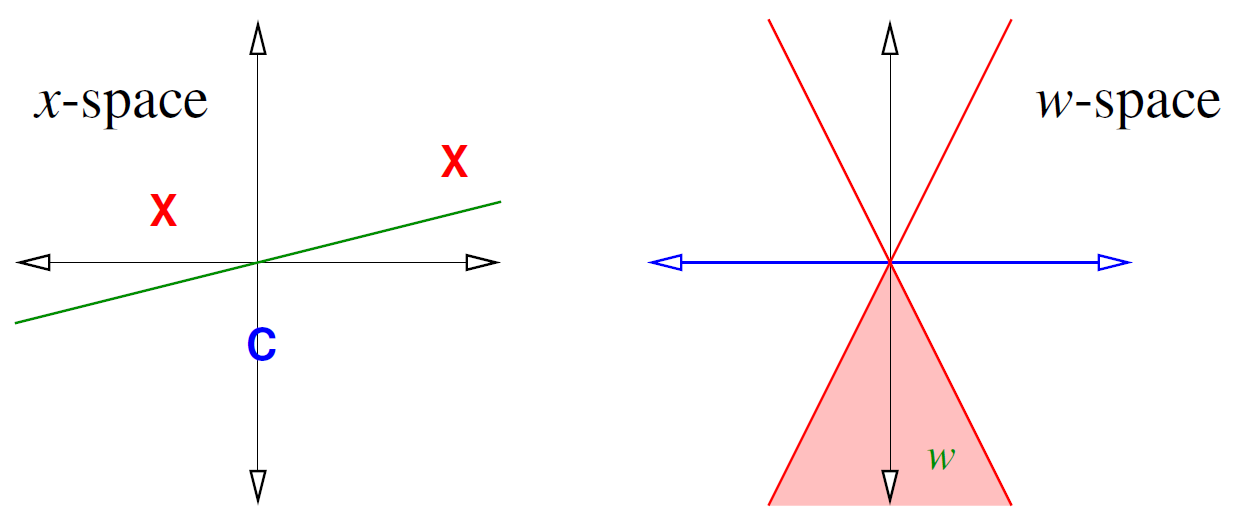
\includegraphics[width=0.4\textwidth]{XSpaceWSpace.PNG}
		\label{XSpaceWSpace}
		\caption{Illustration of how three sample points in x-space (left) can constrain the possible values for w in w space (right).}
	\end{figure}
\end{itemize}

\subsubsection{\green{Algorithm: Gradient Descent}}
\begin{itemize}
	\item GD on our risk function $R$ is an example of an \purple{optimization algorithm}. We want to \textit{minimize} our risk, so we take successive steps in the \textit{opposite} direction of $\nabla R(w)$.\footnote{Recall that the gradient points in direction of steepest \emph{ascent}.}
	\begin{align}
	\nabla R(w) &= \nabla \sum_{i \in V} ( -y_i ~ X_i \cdot w) \\
	&=  -\sum_{i \in V} (y_i ~ X_i )
	\end{align}
	\item \purple{\textbf{Algorithm:}}
	\begin{itemize}
		\item $w \leftarrow $ arbitrary nonzero (e.g. any $y_i X_i$ )
		\item while $R(w) > 0$
		\begin{itemize}
			\item $V \leftarrow $ all $i$ for which $y_i X_i \cdot w < 0$
			\item $w \leftarrow w + \epsilon \sum_{i \in V} (y_i ~ X_i )$
		\end{itemize}
	\end{itemize}
	where $\epsilon$ is the \blue{learning rate/step size}. Each step is $O(nd)$ time.
\end{itemize}

\subsubsection{\green{Algorithm: Stochastic GD}}
\begin{itemize}
	\item Procedure is simply GD on one data point only per step, i.e. no summation symbol. Called the \purple{perceptron algorithm}.
	\item \purple{\textbf{Algorithm:}}
	\begin{itemize}
		\item while some $y_i X_i \cdot w < 0$
		\begin{itemize}
			\item $w \leftarrow w + \epsilon y_i X_i$
		\end{itemize}
		\item return $w$.
	\end{itemize}
	\item \blue{Perceptron Convergence:} If data is linearly separable, perfect linear classifier will be found in at most $O(R^2 / \gamma^2)$ iterations, where
	\begin{itemize}
		\item $R = \max_i |X_i|$ is radius of the data
		\item $\gamma$ is the maximum margin.
	\end{itemize}
\end{itemize}

\subsubsection{\green{Maximum Margin Classifiers}}
\begin{itemize}
	\item \blue{Margin}: (of a linear classifier) the distance from the decision boundary to the nearest sample point.
	\item \purple{Goal}: Make the margin as large as possible.
	\begin{itemize}
		\item Recall that the margin is defined as $|\tau_{min}|$, the magnitude of the smallest euclidean distance from a sample point to the decision boundary, where for some $x_i$,
		\[ \tau_i = \frac{|f(x_i)|}{||w||} \]
		and our goal is to \emph{maximize} the value of the \emph{smallest} $\tau$ in the dataset.
		\item Enforce the (seemingly arbitrary\red{?}) constraints that $|f(x_i)| \ge 1$, or equivalently
		\begin{align}
		y_i (w \cdot x_i + \alpha) \ge 1
		\end{align}
		which can also be stated as requiring all $\tau_i \ge 1/||w||$.
		\item \textbf{Optimize:} Find $w$ and $\alpha$ that minimize $||w||^2$, subject to $y_i (w \cdot x_i + \alpha) \ge 1$ for all $i \in [1, n]$. ``Called a \blue{quadratic program} in d+1 dimensions and n constraints. It has \textbf{one unique solution.}''
	\end{itemize}
	\item The solution is a \blue{maximum margin classifier} aka a \blue{hard SVM}.
\end{itemize}

% =================================================
% Shewchuck Chapter 4
% =================================================
\lecture{Shewchuck Chapter 4}{Soft-Margin SVMs}{}

\begin{itemize}
	\item Hard-margin SVMs fail if not linearly separable.
	\item \purple{Idea:} Allow some points to violate the margin, with \blue{slack variables} $\xi$
	\begin{equation}
	y_i (X_i \cdot w + \alpha) \ge 1 - \xi_i
	\end{equation}
	where $\xi_i \ge 0$. Note that each sample point is \emph{assigned} a value of $\xi_i$, which is only nonzero iff $x_i$ violates the margin.
	\item To prevent abuse of slack, add a \textbf{\blue{loss term}} to our objective function\footnote{Before this, looks like our objective function was just $|w|^2$ since that is what we wanted to minimize (subject to constraints).}.
	\begin{itemize}
		\item Find $w$, $\alpha$, and $\xi_i$ that minimize our objective function,
		\begin{align}
		|w|^2 + C \sum_{i = 1}^n \xi_i
		\end{align}
		subject to
		\begin{align}
		y_i (X_i \cdot w + \alpha) \ge 1 - \xi_i \quad &\text{for all } i \in [1,n] \\
		\xi_i \ge 0 \quad &\text{for all } i \in [1,n]
		\end{align}
		a quadratic program in d + n + 1 dimensions and 2n constraints. The relative size of $C$, the \blue{regularization hyperparameter} determines whether you are more concerned with getting a large margin (small $C$) or keeping the slack variables as small as possible (large $C$).
	\end{itemize}
\end{itemize}

% =================================================
% Shewchuck Chapter 6
% =================================================
\lecture{Shewchuck Chapter 6}{Decision Theory}{}

\begin{itemize}
	\item For when ``a sample point in feature space doesn't have just one class''. Solution is to classify with probabilities.
	\item \blue{Important terminology:}
	\begin{itemize}
		\item \textbf{Loss Function} $L(z, y)$: Specifies badness of classifying as $z$ when the true class is $y$. Can be \blue{asymmetrical}. We are typically used to the \textit{0-1 loss function} which is symmetric: 1 if incorrect, 0 if correct.

		\item \textbf{Decision rule (classifier)} $r : \mathbb{R}^d \rightarrow \pm 1$. Maps feature vector $x$ to a class (1 if in class, -1 if not in class for binary case).

		\item \textbf{Risk}: Expected loss over \textit{all} values of $x$, $y$:
		\begin{align}
			R(r) &= \mathbb{E} \big[ L(r(X), Y) \big]  \\
			&= \sum_y P(Y = y) \sum_x P(X = x | Y = y) L(r(x), y)
		\end{align}
		In ESL Chapter 2.4, this is denoted as the \purple{ prediction error}.

		\item \textbf{Bayes decision rule/classifier} $r*$: Defined as the decision rule $r = r*$ that minimizes $R(r)$. If we assume $L(z, y) = 0$ when $z = y$, then
		\begin{equation}
			r^*(x) = \begin{cases}
				1 & L(-1, 1) P(1 | x) > L(1, 1) P(-1 | x) \\
				-1 & \text{otherwise}
			\end{cases}
		\end{equation}
		which has \textit{optimal risk}, also called the \blue{Bayes risk} $R(r^*)$.
	\end{itemize}

	\item Three ways to build classifiers:
	\begin{itemize}
		\item \blue{Generative models (LDA)}: Assume sample points come frome class-conditioned probability distributions $P(x|c)$, different for each class. Guess the form of these dists. For each class $C$, fit (guessed) distributions to points labeled as class $C$. Also need to estimate (basically make up?) $P(C)$. Use bayes rule and classify on $\max_C P(Y = C|X = x)$. \purple{Advantage}: Can diagnose outliers (small P(x)). Can know the probability that prediction is wrong. \red{Real definition}: A full probabilistic model of all variables.
		\item \blue{Discriminative models}. Model $P(Y|X)$ directly. (I guess this means don't bother with modelling all the other stuff like X|Y, just go for it bruh.) \purple{Advantage:} Can know probability of prediction being wrong. \red{Real definition}: A model only for the target variables.
		\item \blue{Decision boundary finding}: e.g. SVMs. Model $r(x)$ directly. \purple{Advantage}: Easier; always works if linearly separable; don't have to guess explicit distributions.
	\end{itemize}
\end{itemize}


% =================================================
% Shewchuck Chapter 7
% =================================================
\lecture{Shewchuck Chapter 7}{Gaussian Discriminant Analysis}{}

\begin{itemize}
	\item \blue{Fundamental assumption:} Each class C comes from a normal distribution.
	\item For a given $x$, want to maximize $P(X = x | Y = C) \pi_C$, where $\pi_C$ prior probability of class c. Easier to maximize $ln(z)$ since increases monotonically for $z > 0$. The following gives the ``quadratic in x'' function $Q_C(x)$,
	\begin{align}
		Q_C(x)
		&= \ln \bigg( (\sqrt{2 \pi})^d P(x) \pi_C \bigg) \\
		&= -\frac{|x - \mu_C|^2}{2 \sigma_C^2} - d \ln \sigma_C + \ln \pi_C
	\end{align}
	where $P(x)$, a normal distribution, is what we use to estimate the class conditional $P(x|C)$.
	\item The Bayes decision rule $r^*$ returns the class $C$ that maximizes $Q_C(x)$ above.
\end{itemize}

% ---------------- QUADRATIC DISCRIMINANT ANALYSIS ----------------
\subsubsection{\green{Quadratic Discriminant Analysis (QDA)}}
\begin{itemize}
	\item Suppose only 2 classes, C and D. Then
	\begin{equation}
		r^*(x) =
		\begin{cases}
			C & Q_C(x) - Q_D(x) > 0 \\
			D & \text{otherwise}
		\end{cases}
	\end{equation}
	which is quadratic in x. The Baye's Decision Boundary (BDB) is the solution of $Q_C(x) - Q_D(x) = 0$.
	\item In 1D, BDB may have 1 or 2 points (solution to quadratic equation)
	\item In 2D, BDB is a \purple{\textit{quadric}} (e.g. for d=2, conic section).
	\item In 2-class problems, naturally leads to \blue{logistic/sigmoid} function for determining $P(Y|X)$.
\end{itemize}

\subsection{Newton's Method}
\begin{itemize}
	\item Iterative optimization for some smooth function $J(w)$. 
	\item Can Taylor expand gradient about $v$:
	\begin{align}
		\nabla J(w) = \nabla J(v) + (w - v)\nabla^2 J(v) + \mathcal{O}(|w-v|^2)
	\end{align}
	where $\nabla^2 J(v) $ is the \blue{Hessian matrix} of $J(w)$ at $v$, which I'll denote $\matr{H}$. 
	\item Find critical point $w$ where $\nabla J(w) = 0$:
	\begin{align}
		w = v - H^{-1} \nabla J(v)
	\end{align}
	\item Shewchuck defines \blue{Newton's method} algorithm as:
	\begin{enumerate}
		\item Initialize $w$. 
		\item until convergence do:
		\subitem $e := solve\_linear\_system\bigg(\matr{H} e = -\nabla J(w) \bigg)$. 
		\subitem $w := w + e$. 
	\end{enumerate}
	where starting $w$ must be ``close enough'' to desired solution.
\end{itemize}


\subsection{Justifications \& Bias-Variance (12)}
\begin{itemize}
	\item Overview: Describes models, how they lead to optimization problems, and how they contribute to underfitting/overfitting.
	\item Typical model of reality:
	\begin{align}
		y_i = f(X_i) + \epsilon_i
	\end{align}
	where $\epsilon_i \sim D'$ has mean zero. 
	\item Goal of regression: find $h$ that estimates $f$. 
\end{itemize}









% --------------------------------------------------------------------------
% ==========================================================================
% ELEMENTS OF STATISTICAL LEARNING
\newcommand\tlab[1]{\tag{#1}\label{#1}}
% --------------------------------------------------------------------------
% ==========================================================================
\mysection{Elements of Statistical Learning}\label{ESL}

\lecture{ESL}{Linear Regression}{}

\begin{itemize}
	\item Assumption: The \blue{regression function} $\E{Y|X}$ is linear\footnote{or reasonably approximated as linear} in the inputs $X_1, \ldots, X_p$. 
	\item Perform well for\textellipsis
	\begin{itemize}
		\item Small numbers of training cases.
		\item Low signal/noise.
		\item Sparse data. 
	\end{itemize}
\end{itemize}
	
\subsubsection{Models and Least-Squares}
\begin{itemize}
	\item The \blue{model}:
	\begin{align}
		f(X) &= \beta_0 + \jpsum X_j \beta_j \tlab{3.1}
	\end{align}
	
	\item Most popular \blue{estimation method} is least-squares.
	\begin{align}
		RSS(\beta) &= \insum \big(y_i - f(x_i)\big)^2 \tlab{3.2} \\
		&= (\bm{y} - \bm{X}\beta)^T  (\bm{y} - \bm{X}\beta)^T \tlab{3.3}
	\end{align}
	which is reasonable if training observations $(x_i, y_i)$ represent independent random draws from their population\footnote{and/or if $y_i$'s conditionally indep given the $x_i$'s.}.
	
	\item First two derivatives wrt to parameter vector $\beta$:
	\begin{align}
	\begin{split}
		\pderiv{RSS}{\beta} &= -2\bm{X}^T(\bm{y}-\bm{X}\beta) \\
		\frac{\partial^2 RSS}{\partial\beta\partial\beta^T}&= 2\bm{X}^T \bm{X}
	\end{split}
		\tlab{3.4}
	\end{align}
	
	\item Assuming that $\X$ has full column rank so that $\X^T\X$ is positive definite\footnote{A matrix is positive definite if it's symmetric and all its eigenvalues are positive. \red{What would we do here if $X$ were \textit{not} full column rank?}. \green{Answer:} $\X$ columns may not be linearly independent if, e.g., two inputs were perfectly correlated $\matr{x}_2=3\matr{x_1}$. The fitted $\yhat$ will still be projection onto $C(\X)$, but there will be more than 1 way (not unique) to express that projection. Occurs most often when one or more (qualitative) inputs are coded in a redundant fashion.}, set first derive to 0 to obtain the unique solution:\graybox{
			\hat{\beta} = (\X^T\X)^{-1} \X^T \y \tlab{3.6}}
	
	\item \blue{Geometry of Least Squares} \textsc{i get it now!}
	\begin{itemize}
		\item The $(p+1)$ column vectors of $\X$ span a subspace of $\R^N$.\footnote{This is the \red{column space} $C(\X)$ of $\X$. It is the space of $\X v ~ \forall v \in \R^N$, since the produce $Xv$ is just a linear combination of the columns in $X$ with coefficients $v_i$.}. 
		\item Minimizing $RSS(\beta) = \sqnorm{\y - \X\beta}$ is choosing $\hat{\beta}$ such that the \green{residual vector} $\y - \hat{\y}$ is orthogonal to this subspace\footnote{Interpret: $X\beta$ will always lie \textit{somewhere} in this subspace, but we want $\beta$ such that, when we subtract each component (WOAH JUST CLICKED) from the prediction, they cancel exactly,i.e. $y_i-(\X\beta)_i=0$ for all dimensions $i$ in $C(X)$. The resultant vector $\y-\hat{y}$ will only contain components outside this subspace, hence it is orthogonal to it by definition.}. Stated another way, (the optimal) $\hat{y}$ is the \textit{orthogonal projection of $\y$ onto the column space of $X$}. 
		\item Since $\yhat = \X\bhat$, we can define this projection matrix (aka hat matrix), denoted as $\matr{H}$, where
		\begin{align}
		\begin{split}
			\yhat &= \X\bhat \\
			&= \X(\X^T\X)^{-1}\X^T\y \\
			&= \matr{H}\y
		\end{split}
		\tlab{3.7}
		\end{align}
	\end{itemize}
\end{itemize}

\p \Part{Why $Var(\hat{\beta}) = (\X^T\X)^{-1}\sigma^2$.}
\begin{itemize}
	\item Note: \blue{Variance-covariance matrix} $\equiv$ Covariance matrix.
	\item Can express the \blue{correlation matrix} in terms of the covariance matrix:
	\begin{align}
		corr(\X) &= \big( diag(\Sigma)\big)^{-1/2}  \Sigma \big( diag(\Sigma)\big)^{-1/2}
	\end{align}
	or, equivalently, the correlation matrix can be seen as the covariance matrix of the standardized random variables $X_i/\sigma(X_i)$. 
	\item Recall from decision theory that, when we want find a function $f(X)$ for predicting some $Y \in \R$, we can do this by \textit{minimizing the risk} (aka the  prediction error EPE(f)). This is accomplished first by defining a loss function. Here we will use the squared error loss $L(Y, f(X)) = (Y - f(X))^2$. We can express $EPE(f)$ as an integral over all values that $Y$ and $X$ may take on (i.e. the joint distribution). Therefore, we can factor the joint distribution and define $f(x)$ via minimizing EPE piecewise (meaning at each value of $X = x$.) This whole description is written mathematically below.
	\begin{align}
		EPE(f) &= \E{Y - f(X)}^2 \tlab{2.9} \\
		&= \int \big[y - f(x) \big]^2 f_{XY}(x, y) dx dy \tlab{2.10} \\
		&= \mathbb{E}_X\Big[ 	\mathbb{E}_{Y|X} \bigg[  (Y - f(X))^2 | X \bigg]	 \Big] \tlab{2.11}
	\end{align}
	and therefore, the best predictor of $Y$ is a function $f:\R^p \rightarrow \R$ that satisfies, for each $x$ value separately
	\begin{align}
		f(x) &= \argmin_{c} \mathbb{E}_{Y|X}  \bigg[  (Y - c)^2 | X \bigg] \tlab{2.12} \\
		&= \E{Y | X = x} \tlab{2.13}
	\end{align}
	which essentially defines what is meant by $\E{Y | X = x}$, also referred to as the \blue{conditional mean}\footnote{At the same time, don't forget that least-squared error assumption was built-in to this derivation.}.
	
	 \redbox[Bias-Variance Tradeoff]{The  test MSE, for a given value $x_0$, can always be decomposed into the sum of three fundamental quantities:
		\begin{align}
			\E{y_0 - \hat{f}(x_0)}^2 = Var\big( \hat{f}(x_0) \big) 
			+ \big[ Bias(\hat{f}(x_0)) \big]^2
			+ Var(\epsilon)
		\end{align}
		which is interpreted as the \textit{ test MSE}: the average test MSE that we would obtain if we repeatedly estimated $f$ using a large number of training sets, and \emph{tested each at $x_0$}. The \textbf{overall test MSE} can be computing the average (of this average) over all possible values of $x_0$ in the TEST set.
	}
	
	\item What \blue{bias} means here: \begin{footnotesize}
		On the other hand, bias refers to the error that is introduced by approximating
		a real-life problem, which may be extremely complicated, by a much
		simpler model. For example, linear regression assumes that there is a linear
		relationship between Y and $X_1, \ldots, X_p$. It is unlikely that any real-life
		problem truly has such a simple linear relationship, and so performing linear
		regression will undoubtedly result in some bias in the estimate of f. In
		Figure 2.11, the true f is substantially non-linear, so no matter how many
		training observations we are given, it will not be possible to produce an
		accurate estimate using linear regression. In other words, linear regression
		results in high bias in this example. However, in Figure 2.10 the true f is
		very close to linear, and so given enough data, it should be possible for
		linear regression to produce an accurate estimate. Generally, more flexible
		methods result in less bias.
	\end{footnotesize}
	
	\item Returning now to the case where know (aka assume) that the true relationship between $X$ and $Y$ is linear
	\begin{align}
		Y = X^T \beta + \epsilon \tlab{2.26}
	\end{align}
	and so \textit{in this particular case} the least squares estimates are \emph{unbiased}. 
	
	\item This is the proof: (relies on the fact that $Var(\beta) = 0$ since $\beta$ is the \emph{true} (NON RANDOM) vector we are estimating)\footnote{Also, $\forall a \in \R: Var(a + X) = Var(X)$}
	\begin{align}
		Var[\hat{\beta}] &= Var\bigg[ (\X^T \X)^{-1} \X^T \y	\bigg] \\
		&= Var\bigg[ (\X^T \X)^{-1} \X^T \big( \X \beta + \epsilon  \big)	\bigg] \\
		&= Var\bigg[ (\X^T \X)^{-1} \X^T  \X \beta +  (\X^T \X)^{-1} \X^T \epsilon  	\bigg] \\
		&= Var\bigg[ \beta +  (\X^T \X)^{-1} \X^T \epsilon  	\bigg] \\
		&= Var\bigg[ (\X^T \X)^{-1} \X^T \epsilon  	\bigg] \\
		&= \mathbb{E}\Big[	\bigg( 	(\X^T \X)^{-1} \X^T \epsilon	\bigg) \bigg(	(\X^T \X)^{-1} \X^T \epsilon \bigg)^T	\Big] \\
		&= 	\bigg( 	(\X^T \X)^{-1} \X^T  \bigg)  ~ \E{\epsilon\epsilon^T} ~ \bigg( \X 	(\X^T \X)^{-1}   \bigg)	\\
		&= 	\bigg( 	(\X^T \X)^{-1} \X^T  \bigg)  ~ \sigma^2 ~ \bigg( \X 	(\X^T \X)^{-1}   \bigg)	 \\
		&= \sigma^2	\bigg( 	(\X^T \X)^{-1} \X^T  \bigg)  \bigg( \X 	(\X^T \X)^{-1}   \bigg)	 \\
		&= \sigma^2	 	(\X^T \X)^{-1}
	\end{align}
	where we have assumed that the $X$ are FIXED (not random)\footnote{another way of stating this is that we took the variance \emph{given} (or conditioned on) each $X$} and so the variance of (some product of $X$s) $\times$ $\epsilon$ is like taking the variance with a constant out front. We've also assumed that $X^T X$ (and thus its inverse too) is symmetric, apparently. 
\end{itemize}

\subsubsection{Subset Selection (3.3)}
\begin{itemize}
	\item Two reasons why we might not be satisfied with ~\ref{3.6}:
	\begin{enumerate}
		\item Prediction accuracy. Often have low bias, high variance. May improve if shrink coefficients. Sacrifices some bias to reduce variance. 
		\item Interpretation. Sacrifices some of the small details.
	\end{enumerate}
	\item Appears that subset selection refers to retaining a subset of the \textit{predictors} $\bhat_i$ and discarding the rest.
	\item Doing this can often exhibit high variance, even if lower prediction error. 
\end{itemize}

\subsubsection{Shrinkage Methods (3.4)}
\begin{itemize}
	\item Shrinkage methods are considered \textit{continuous} (as opposed to subset selection) and don't suffer as much from high variability. 
\end{itemize}



% ====================================================================
% ====================================================================
\lecture{ESL}{Linear Methods for Classification (Ch. 4)}{July 30, 2017}
% ====================================================================
% ====================================================================


\p \blue{Logistic Regression} (4.4). Motivation: we want to model $\Prob{G = k \mid X = x}$, for each of our $K$ classes, via \underline{linear functions in x}. 
\graybox{
	\log \dfrac{ \Prob{G = k \mid X = x}  }{  \Prob{G = K \mid X = x} } &= (\beta_0)_k + \beta_{k}^T x \qquad \forall k \in [1, K-1] \\
	\Prob{G = k \mid X = x} &= \dfrac{ e^{ \beta_{0k} + \beta_{k}^T x}   }{ 
		 1 + \sum_{\ell = 1}^{K - 1} e^{ \beta_{0\ell} + \beta_{\ell}^T x}  } \quad \forall k \in [1, K-1] \\
		&\triangleq p_k(x;\theta) 
	}
where $\theta \triangleq \{\beta_{01}, \beta_1^T, \ldots, \beta_{(K-1)0}, \beta_{K-1}^T \}$. 


% ====================================================================
% ====================================================================
\lecture{ESL}{Naive Bayes}{}
% ====================================================================
% ====================================================================


\p Appropriate when dimension $p$ of feature space is large. It assume that given a class $G = j$, the features $X_k$ are independent:
\begin{align}
	f_j(X) \equiv f_j((X_1, X_2, \ldots, X_p)^T) = \prod_{k = 1}^{p} f_{jk}(X_k)
\end{align}
which can simplify estimation [of the class-conditional probability densities $f_j(X)$] dramatically: The individual class-conditional marginal densities $f_{jk}$ can each be estimated \textit{separately} using 1D kernel density estimates. 

\lecture{ESL}{Trees and Boosting}{}

\myspace
\hrule
\subsubsection{Boosting Methods (10.1)}

\p \blue{Terminology}:
\begin{compactitem}
	\item \textbf{Weak Classifier}: one whose error rate is only slightly better than random guessing.
\end{compactitem}

\p \blue{The AdaBoost algorithm}. 

\begin{enumerate}
	\item Initialize observation weights $w_i := 1/N$, $i = 1, 2, \ldots, N$. 
	
	\item For $m = 1$ to $M$\footnote{where $M$ is the number of weak classifiers (trees) that we want to train.}:
	\begin{enumerate}
		\item Fit classifier $G_m(x)$ to the training data using weights $w_i$. 
		\item Compute
		\graybox{
			\text{err}_m = \dfrac{\sum_{i = 1}^{N} w_i I(y_i \ne G_m(x_i)) 	}{ \sum_{i = 1}^{N} w_i}
			}
		\item Compute $\alpha_m = \log\left( (1 - \text{err}_m)/\text{err}_m \right)$.
		\item Update $w_i \leftarrow w_i \cdot \exp[ \alpha_m \cdot I(y_i \ne G_m(x_i)) ]$, $i = 1, \ldots, N$.
	\end{enumerate}
	
	\item Output $G(x) = \sum_{i = 1}^{m} \alpha_m G_m(x)$. 
\end{enumerate}
\hrule


\lecture{ESL}{Basis Expansions and Regularization (Ch 5)}{}

\p \blue{Introduction}. Core idea is to augment/replace the vector of inputs $X$ with additional variables, which are transformations of $X$, and then use linear models in this new space of derived inputs features. Specifically, we model a \textit{linear basis expansion} in $X$:\marginnote{$h_m(X) : \R^p \rightarrowtail \R$.}[3em]
\graybox{
	f(X) &= \sum_{m = 1}^{M} \beta_m h_m(X)
	}
where $h_m(X)$ is the $m$th transformation of $X$, $m = 1,\ldots,M$. 

\myspace
\p \blue{Piecewise Polynomials and Splines}. Assume that $X$ is one-dimensional. We will explore increasingly complex cases that build off each other.
\begin{compactitem}
	\item \textbf{Piecewise-constant}. Take, for example, the case where we have 3 basis functions:
	\begin{align}
		h_1(X) = I(X < \xi_1), \quad h_2(X) = I(\xi_1 \le X < \xi_2), \quad h_3(x) = I(\xi_2 \le X) \label{piecewise-basis}
	\end{align}
	Solving for $\beta_i$ in each derivative of $RSS(\beta)$ w.r.t. $\beta_i$, for $f(X) = \sum_{i = 1}^{3} \beta_i h_i(X)$, yields $\hat \beta_i = \bar Y_i$, the mean of $Y$ in the $i$th (of 3) regions. Note that this is the \underline{degree-0 case}: piecewise constant. \\
	
	\item \textbf{Piecewise-linear}. Instead of just learning the best-fit constant $\beta_i$ for the $i$th region, we can now also learn the best \textit{slope} for the line in that region. This means we have 3 additional parameters to fit, and $f(X)$ becomes:
	\begin{align}
		f(X) &= \beta_1 I_1 + \beta_2 I_2 + \beta_3 I_3 + \beta_4 I_1 \cdot X + \beta_5 I_2 \cdot X + \beta_6 I_3 \cdot X \\
		&= (\beta_1 + \beta_4 X) I_1 + (\beta_2 + \beta_5 X) I_2 + (\beta_3 + \beta_6 X) I_3
	\end{align}
	where I've denoted the $i$th identity function from \ref{piecewise-basis} as $I_i$. 
	
	\item \textbf{Continuous piecewise-linear}. We would typically prefer the lines to meet (have the same value) at the region boundaries of $X = \xi_1$ and $X = \xi_2$. In other words, require that:
	\begin{align}
		f(\xi_1^-) = \beta_1 + \beta_4 \xi_1 &= \beta_2 + \beta_5 \xi_1 = f(\xi_1^+) \\
		f(\xi_2^-) = \beta_2 + \beta_5\xi_2 &= \beta_3 + \beta_6 \xi_2 = f(\xi_2+)
	\end{align}
	which also reduces our free parameters from 6 to 4\footnote{Because, for example, now $\beta_1 = \beta_2 + (\beta_5 - \beta_4) \xi_1$.}. We can express this constraint more directly by using a basis that incorporates them\footnote{Note: I was not able to derive this form from the previous equations and constraints. Moving on because not important right now.}. 
	\begin{align}
		h_1(X) = 1, \quad h_2(X) = X, \quad h_3(X) = (X - \xi_1)_+, \quad h_4(X) = (X - \xi_2)_+
	\end{align}                                               
\end{compactitem}
In general, \textbf{an order-$M$ spline with knots $\xi_j, ~ j = 1,\ldots,K$ is a piecewise-polynomial of order $M$, and has continuous derivatives up to order $M-2$}. 

\myspace
\p \blue{B-splines}. Let $\xi_0$ and $\xi_K$ denote two \textbf{boundary knots}, which typically define the domain over which we wish to evaluate our spline. Define the augmented knot sequence $\tau$ such that\marginnote{It is customary to make all $\tau_{i, i \le M} = \xi_0$ and $\tau_{j, j \ge K + M + 1} = \xi_{K + 1}$.}[2em]
\begin{align}
	&\tau_i \le \tau_2 \le \cdots \le \tau_M \le \xi_0 \\
	&\tau_{M + j} = \xi_j, ~ j = 1, \cdots, K \\
	&\xi_{K + 1} \le \tau_{K + M + 1} \le \tau_{K + M + 2} \le \cdots \le \tau_{K + 2M}
\end{align}
The $i$th $B$-spline basis function of order $m$ ($m \le M$) for the knot sequence $\tau$ is denoted by $B_{i,m}(x)$, and defined recursively as follows:
\graybox{
	B_{i,1}(x) &= \begin{cases}
		1 & \tau_i \le x \le \tau_{i + 1} \\
		0 & \text{otherwise}
	\end{cases} \quad i=1,\ldots,K+2M-1\\
	B_{i,m}(x) &= 
		\tfrac{x - \tau_i}{\tau_{i+m-1} - \tau_i} B_{i,m-1}(x) +
		\tfrac{\tau_{i+m} - x}{\tau_{i+m} - \tau_{i+1}} B_{i+1,m-1}(x)
		\quad i=1,\ldots,K+2M-m
	}



% ==============================================================================================
\lecture{ESL}{Model Assessment and Selection (Ch. 7)}{}

\p \blue{Bias, Variance, and Model Complexity}. We first define the three main quantities:
\graybox{
	\mtgreen{Generalization (Test) Error} \qquad \text{Err}_{\mathcal{T}} &= \E{L(Y, \hat f (X)) \mid \mathcal{T}} \\
	\mtred{Expected Prediction Error} \qquad \text{Err} &= \E{L(Y, \hat f (X))} = \E{\text{Err}_{\mathcal{T}}} \\
	\mtgreen{Training Error} \qquad \overline{\text{err}} &= \frac{1}{N} \sum_{i=1}^{N} L(y_i, \hat f (x_i))
}

\myfig[0.5\textwidth]{figs/BiasVarianceComplexity.png}


\myspace
\p \blue{Bias-Variance Decomposition}. Let $Y = f(X) + \varepsilon$, $\E{\epsilon} = 0$, $\Var{\varepsilon} = \sigma_\varepsilon^2$. We derive the expected prediction error of a fit $\hat f (X)$ at an input point $X = x_0$, using squared-error loss:\marginnote{$\varepsilon$ and $\hat f$ are independent.}[6em]
\begin{align}
	\text{Err}(x_0) &= \E[\varepsilon, \hat f]{(Y - \hat f (x_0))^2 \mid X=x_0} \\
	&= \E[\varepsilon, \hat f]{(f - \hat f (x_0) + \varepsilon)^2} \\ 
	&= \E[\varepsilon]{\varepsilon^2} + \E[\hat f]{(f - \hat f (x_0))^2} \\
	&= \sigma_\varepsilon^2 + \E[\hat f]{\hat f (x_0)^2} + f^2 - 2f\E[\hat f]{\hat f (x_0)} \\
	&= \sigma_\varepsilon^2 + \E[\hat f]{\hat f (x_0)^2} \mgreen{
			- \E[\hat f]{\hat f (x_0)}^2 + \E[\hat f]{\hat f (x_0)}^2
			}
		+ f^2 - 2f\E[\hat f]{\hat f (x_0)} \\
	&= \sigma_\varepsilon^2 + \Var{\hat f (x_0)} + \left( \E[\hat f]{\hat f (x_0)}^2 - 2f \E[\hat f]{\hat f (x_0)} + f^2\right) \\
	&= \sigma_\varepsilon^2 + \Var{\hat f (x_0)} + \left(\E[\hat f]{\hat f (x_0)} - f\right)^2 \\
	&=  \sigma_\varepsilon^2 + \Var{\hat f (x_0)} + \text{Bias}^2\left(\hat f (x_0) \right)
\end{align}
Remember, $\text{Err}(x_0)$ is the MSE of the prediction at $X = x_0$, taken over all possible models $\hat f$ (and the irreducible error from $\varepsilon$). The bias is the difference between the average estimate, $\E[\hat f]{\hat f (x_0)}$, and the true mean of Y, $f(x_0)$. Finally, the variance measures how much the distribution over all possible $\hat f$ deviates from their average, $\E[\hat f]{\hat f (x_0)}$. 

\myspace
\p \blue{Bootstrap Methods}. A general tool for assessing statistical accuracy. Seeks to estimate the conditional error $\text{Err}_{\mathcal{T}}$ but typically estimates well only the expected prediction error $\text{Err}$. Denote our training set $\mathcal{T}$ by $\matr{Z} = (z_1, \ldots, z_N)$, where $z_i = (x_i, y_i)$. The basic procedure is as follows:
\begin{compactenum} 
	\item We randomly draw datasets with replacement from $\matr{Z}$, with each sampled dataset, $\matr{Z}^{*b}$, having the same size, $N$, as $\matr{Z}$. 
	
	\subitem- This is done $B$ times, producing $B$ bootstrap datasets.
	
	\item Refit the model to each of the bootstrap datasets, and examine the behavior of the fits over the $B$ replications.
\end{compactenum}

% \lecture{ESL}{Model Inference and Averaging (Ch. 8)}{}
%
% \p \blue{Bootstrap and Maximum Likelihood Methods}. 


% --------------------------------------------------------------------------
% --------------------------------------------------------------------------
% ==========================================================================
% Concept Summaries
% --------------------------------------------------------------------------
% --------------------------------------------------------------------------
% ==========================================================================
\mysection{Concept Summaries}\label{Concept Summaries}


\lecture{Concept Summaries}{Probability Review}{}

\p \blue{Notation}:\vspace{-1em}
\begin{itemize}[--]
	\item \green{Sample Space} $\Omega$: Set of all outcomes of a random experiment. For six-sided die, $\Omega = \{1, \ldots, 6\}$. 
	\item \green{Event Space} $\F$: Set whose \textit{elements} are \textit{subsets} of $\Omega$. Appears that $\F$ is required to be complete in a certain sense, i.e. that it should contain \textit{all} possible events (combinations of possible individual outcomes). 
	\item \green{Probability measure}: Function $P : \F \rightarrow \R$. Intuitively, it tells you what fraction of the total space of possibilities that $\F$ is in, where if $\F$ \textit{is} the full space, $P(F) = P(\Omega) = 1$. Also required: $P(A) \ge 0 ~~ \forall A \in \F$. 
\end{itemize}

\myspace
\p \blue{Random Variables}:\footnote{TIL I had no idea what a random variable really was.}\vspace{-1em}
\begin{itemize}[--]
	\item Consider experiment: Flip 10 coins. An example element of $\Omega$ would be of the form 
	\begin{align}
	\omega_0 = (H, H, T, H, T, H, H, T, H, T) \in \Omega
	\end{align}
	which is typically a quantity too specific for us to really care about. Instead, we prefer real-valued \textit{functions} of outcomes, known as \blue{random variables}. 
	\item R.V. $X$ is defined as a function $X: \Omega \rightarrow \R$. They are denoted as $X(\omega)$, or simply $X$ if $\omega$ dependence is obvious. 
	\item Using our definition of the probability measure, we define the probability that $X = k$ as the probability measure over the space containing all outcomes $\omega$ where $X(\omega) = k$.\footnote{Oh my god yes, this is what I came here for.} \graybox{
		P( X = k) := P(\{\omega : X(\omega) = k \})
}
	
	\item \green{Cumulative Distribution Function:} $F_X : \R \rightarrow [0, 1]$ defined as\footnote{The symbol $\triangleq$ means equal by definition (hnnggg). In continuous case, $F_X(x) = \int_{-\infty}^{x} p_X(u) du$.}
	\begin{align}
	F_X(x) \triangleq P(X \le x)
	\end{align}
	
	\item \green{Probability Mass Function}: When $X$ is a \textit{discrete} RV, it is simpler to represent the probability measure by directly saying the probability of each possible value $X$ can assume. It is a function $p_X : \Omega \rightarrow \R$ such that 
	\begin{align}
	p_X (x) \triangleq P(X = x)
	\end{align}
	
	\item \green{Probability Density Function}: The derivative of the CDF. 
	\begin{align}
	f_X (x) &\triangleq \deriv{F_X(x)}{x} \\
	P(x \le X \le x + \delta x) &\approx f_x(x) \delta x
	\end{align}
\end{itemize}

\myspace
\p \blue{Expectation Values}\vspace{-1em}
\begin{itemize}[--]
	\item Discrete $X$: (PMF $p_X(x)$) Can either take expectations of $X$ (the mean) or of some function $g(X): \R \rightarrow \R$, also a random variable.\graybox{
		\E{g(X)} &\triangleq \sum_{x \in Val(X) } g(x) p_X(x) \\
		\E{X} &\triangleq \sum_{x \in Val(X) } x p_X(x) 
	}
	
	\item Continuous $X$: (PDF $f_X(x)$), then 
	\begin{align}
	\E{g(X)} \triangleq \int_{-\infty}^{\infty} g(x) f_X(x) \mathrm{d}x
	\end{align}
	
	\item \textbf{Properties}:
	\begin{align}
	\E{a} 		&= a \quad \forall a \in \R \\
	\E{a~f(X)} 	&= a \E{f(X)} \\
	\E{f(X) + g(X)} &= \E{f(X)} + \E{g(X)} \\
	\E{bool(X == k)} &= P(X = k)
	\end{align}
\end{itemize}

\myspace
\p \blue{Variance}: Measure of how concentrated the dist of a RV is around its mean. 
\begin{align}
Var[X] &\triangleq \E{(X - \E{X})^2} \\
&= \E{X^2} - \E{X}^2
\end{align}
with properties:
\begin{align}
Var[a] &= 0 \quad \forall a \in \R \\
\varDelta[a f(X)] &= a^2 Var[f(X)]
\end{align}

\myfig{CommonRandomVariables.PNG}

\p \blue{Covariance}\vspace{-1em}
\begin{itemize}[--]
	\item Recognize that the covariance of two random variables $X$ and $Y$ can be described as a \textit{function} $g: \R^2 \rightarrow \R$. Below we define the expectation value for some multivariable function\footnote{Discrete case shown only. Should be obvious how it would look for continuous.}, and then we can define the covariance as a particular example. \graybox{
		\E{g(X, Y)} &\triangleq \sum_{x \in Val(X)}\sum_{y \in Val(Y)} g(x, y) p_{XY}(x, y) \\
		Cov[X, Y] &= \E{ (X - \E{X}) (Y - \E{Y}) }
	}
	\item Properties:
	\begin{align}
	Cov[X, Y] &= \E{XY} - \E{X}\E{Y} \\
	Var[X + Y] &= Var[X] + Var[Y] + 2Cov[X, Y]
	\end{align}
\end{itemize}

\myspace
\p \blue{Random Vectors}\vspace{-1em}
\begin{itemize}[--]
	\item Suppose we have $n$ random variables $X_i = X_i(\omega)$ all over the same general sample space $\Omega$. Convenient to put them into a \blue{random vector} $X$, defined as $X: \Omega \rightarrow \R^n$ and with $X = [X_1 X_2 \ldots X_n]^T$.
	\item Let $g$ be some function $g: \R^n \rightarrow \R^m$. We can define expectations with notation laid out below. 
	\begin{align}
	\begin{split}
	g(X) = 
	\begin{bmatrix}
	g_1(X) \\
	g_2(X) \\
	\vdots \\
	g_m(X)
	\end{bmatrix}
	\end{split}
	\begin{split}
	\E{g(X)} = 
	\begin{bmatrix}
	\E{g_1(X)} \\
	\E{g_2(X)} \\
	\vdots \\
	\E{g_m(X)}
	\end{bmatrix}
	\end{split}
	\end{align}
	
	\begin{align}
	\E{g_i(X)} = \int_{\R^n} g(x_1,\ldots, x_n)f_{X_1, \ldots, X_n} dx_1\ldots dx_n
	\end{align}
	
	\item For a given $X:\Omega \rightarrow \R^n$, its \textsc{\blue{covariance matrix $\Sigma$}} is the $n \times n$ matrix with $\Sigma_{ij} = Cov[X_i, X_j]$. Also, \graybox{
		\Sigma &= \E{XX^T}- \E{X}\E{X}^T \\
		&= \E{(X - \E{X})(X - \E{X})^T}
	}
	and it satisfies: (1) $\Sigma \succeq 0$ (pos semi-def), (2) $\Sigma$ is symmetric.
\end{itemize}

% --------------------------------------------------------------------------
% ==========================================================================
% MIDTERM STUDYING
% --------------------------------------------------------------------------
% ==========================================================================
\lecture{Concept Summaries}{Commonly Used Matrices and Properties}{}

\begin{tabular}[h]{l l}
	\toprule\toprule
	Matrix & Properties \\ \midrule
	$\left(XX^T + \mu I_n\right)$ 			& P.D. with real eigvals $\lambda_i > $ when $\mu > 0$.  \\
	p.s.d $A$, $B$.							& Product $AB$ NOT guaranteed p.s.d. \\
	$C = [A \circ B]_{ij} = A_{ij}B_{ij}$	& C is p.s.d. (A,B still p.s.d from above)\\
	\bottomrule\bottomrule
\end{tabular}

\myspace
\p \blue{Positive Semi-definite}. 
\begin{compactitem}
	\item Eigenvalues non-negative.
\end{compactitem}

% --------------------------------------------------------------------------
% ==========================================================================
% MIDTERM STUDYING
% --------------------------------------------------------------------------
% ==========================================================================
\lecture{Concept Summaries}{Midterm Studying}{}

\p The eigenvalues of a matrix are the zeros of its \blue{characteristic polynomial}, defined as $f(\lambda) = \det(A - \lambda I)$. A vector $v \ne 0$ is an \blue{eigenvector} iff $v \in Null(A - \lambda I)$.  \\

\p Regardless of offset of plane, the normal vector to ax + by + cz = d is $w = (a, b, c)$. For any point $A$ not on the plane, closest point $B$ to $P$ where $B$ \textit{is} on the plane, is determined by the value of $\alpha$ that solves
\begin{align}
(A - \alpha (a, b, c)) \cdot (a, b, c) = d
\end{align}
since, given $\alpha$ satisfies the equation, $B = (A - \alpha (a, b, c))$ is a point on the plane, constructed by following the direction of $w$ ``backwards'' from $A$.  \\

\p Direct comparison between MLE and \blue{MAP}:\footnote{MAP also known as Bayesian Density Estimation}
\begin{footnotesize}
	\begin{align}
	\begin{split}
	\theta_{MLE} &= \argmax_{\theta} \sum_i \log\big( \mgreen{ p_X(x|\theta) } \big) 
	\end{split}
	\begin{split}
	p(\theta|x) &\propto  \mgreen{p_X(x|\theta)}  p(\theta) \\
	\theta_{MAP} &= \argmax_\theta \sum_i \log\bigg(\mgreen{p_X(x|\theta)}p(\theta)\bigg) \\
	&= \argmax_{\theta}  \E{\log\big[\mgreen{p_X(x|\theta)}\big] + p(\theta) }
	\end{split}
	\end{align}
\end{footnotesize}

% --------------------------------------------------------------------------
% ==========================================================================
% MIDTERM STUDYING
% --------------------------------------------------------------------------
% ==========================================================================
\lecture{Concept Summaries}{Support Vector Machines (CS229)}{}


\begin{itemize}
	\item Note that (logistic regression) 
	\begin{align}
	g(\theta^T) \ge 0.5 \iff \theta^Tx \ge 0
	\end{align}
	\item Switch to perceptron algorithm where 
	\begin{align}
	h_{w, b}(x) = g(w^T x + b) = 
	\begin{cases}
	1 &  w^Tx + b \ge 0 \\
	-1 & \text{otherwise} 
	\end{cases}
	\label{perceptron}
	\end{align}
	\item Given a training example $(x^{(i)}, y^{(i)})$, define the \blue{functional margin} of $(w,b)$ w.r.t the training example as 
	\graybox{
		\hat{\gamma}^{(i)} &= y^{(i)} (w^T x^{(i)} + b)
	}
	where $\hat{\gamma}^{(i)} > 0$ means prediction is correct.\footnote{Possible insight relating to regularization: Notice how perceptron classification $g(x)$ only depends on the sign of it's argument, and not on the \textit{magnitude}. However, performing $x \rightarrow 2x$ causes our functional margin to double $\hat{\gamma}^{(i)} \rightarrow 2 \hat{\gamma}^{(i)}$ and so it seems ``\textit{we can make the functional margin arbitrarily large without really changing anything meaningful.} This leads to, perhaps, defining a normalization condition that $||w||_2 = 1$. Hmmm\textellipsis} We can also define with respect to $S = \{(x^{(i)}, y^{(i)}) : i = 1,\ldots,m \}$ to be the \textit{smallest} of the individual functional margins:
	\begin{align}
	\hat{\gamma} &= \min_{i=1,\ldots,m} \hat{\gamma}^{(i)}
	\end{align}
	\myspace
	
	\item Now we move to \blue{geometric margins}. First, consider figure~\ref{Hyperplane}\footnote{Alright retard, time to settle this once and for all. The plane containing point $P_0$ and the vector $\bm{n} =(a, b, c)$ consists of all points $P$ with corresponding position vector $\bm{r}$ such that the vector drawn from $P_0$ to $P$ is perpendicular to $\bm{n}$, i.e. the plane contains all points $\bm{r}$ such that $\bm{n} \cdot (\bm{r} - \bm{r_0}) = 0$ }
	\begin{figure}[h]
		\centering
		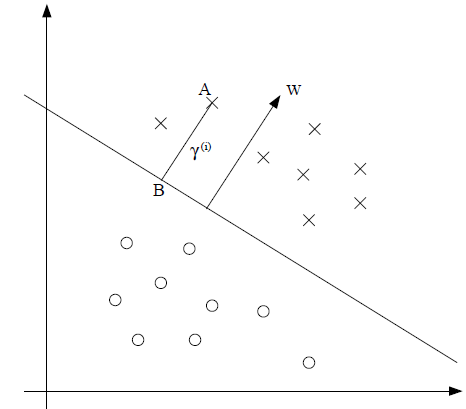
\includegraphics[width=0.2\textwidth]{Hyperplane.PNG}
		\caption{Decision boundary}
		\label{Hyperplane}
	\end{figure}
	
	\item If we consider $A$ as the $i$th data point, what is value of $\gamma^{(i)}$? The point $B$ that is closest to $A$ on the plane is given by $A - \tau \cdot w/||w||$ where $\tau$ is the distance $|AB|$ that we want to solve for. Since $B$ is on the plane, we can solve for $\tau$ via
	\begin{align}
	0 &= w^T \bigg(x^{(i)} - \tau \frac{w}{||w||} \bigg) + b  \\
	\tau &= \frac{w^T x^{(i)}+ b}{||w||}
	\end{align}
	which leads to the general definition for the \textbf{\blue{geometric margin}}, denoted \textit{without the hat} $\gamma^{(i)}$ as 
	\graybox{
		\gamma^{(i)} &= y^{(i)} \bigg[\bigg(\frac{w}{||w||} \bigg)^T x^{(i)} + \frac{b}{||w||}	\bigg]
	}
	where clearly if $||w||=1$ is the same as the functional margin. Also can define the geometric over the whole training set similarly as was done for the functional margin. 
	
	\item \Part{Optimizing (maximizing) the margin}. 
	\begin{itemize}
		\item Pose the following optimization problem
		\begin{align}
		\max_{\gamma, w, b}& ~ \frac{\hat{\gamma}}{||w||} ~~ \mred{S.T.} \\
		y^{(i)} \bigg(w^T x^{(i)}+ b\bigg)& \ge \hat{\gamma} 
		\end{align}
		
		\item Due to reasons primarily regarding how computing $||w||$ is non-convex/hard, we translate the problem as follows: (1) impose (on the \textit{functional margin}\footnote{Recall that the functional margin alone does NOT tell you a distance.}) constraint that\footnote{Also remember that $\hat{\gamma}$ is over the WHOLE training set, and evaluates to the smallest $\hat{\gamma}^{(i)}$}, $\hat{\gamma} = 1$ which we can always satisfy with some scaling of $w$ and $b$; (2) Instead of maximizing $1/||w||$, minimize $||w||^2$. 
		\begin{align}
		\min_{\gamma, w, b}& ~ \onehalf ||w||^2 ~~ \mred{S.T.} \\
		y^{(i)} \bigg(w^T x^{(i)}+ b\bigg)& \ge 1
		\end{align}
		which gives us the \blue{optimal margin classifier}.
		
		\item Lot of subtleties: For SVM (at least in this class) we want maximize the margin, which we \textbf{define} to be $2/||w||$. Note that this is \textit{not} a fixed scalar value, it changes as $||w||$ changes! The \blue{support vectors} are any points $x^{(i)}$ such that $y^{(i)}(w^T x^{(i)} + b) = 1$. 
	\end{itemize}
\end{itemize}
\myspace 

% ____________ legendary proof. author: me ______________
\p \begin{footnotesize} \textbf{\red{PROOF THAT W IS ORTHOGONAL TO THE HYPERPLANE}}
	\begin{itemize}
		\item Claim: If $w$ is a vector that classifies according to perceptron algorithm (equation~\ref{perceptron}), then $w$ is orthogonal to the separating hyperplane. 
		\item Proof: We proceed, using only the definition of a plane, by finding the plane that $w$ is orthogonal to, and show that this plane must be the separating hyperplane. 
		\item If we plug in $w$ to the \textit{point-normal form} of the equation of a plane, \textbf{defined} as the plane containing all points  $\bm{r }= (x, y, z)$ such that $w$ is orthogonal to the \textbf{PLANE}\footnote{NOTE HOW I SAID PLANE AND NOT ANY VECTOR POINTING TO SOME POINT IN THE PLANE}
		\begin{align}
		w_x x + w_y y + w_z z + d &= 0 \\
		\bm{w}^T \bm{r} + d &= 0 \\
		\end{align}
		where, denoting $\bm{r}_0= (x_0, y_0, z_0)$ as the vector pointing to some arbitrary point $P_0$ in the plane,
		\begin{align}
		d &= -(w_x x_0 + w_y y_0 + w_z z_0 ) \\
		&=  - (\bm{w}^T \bm{r}_0)
		\end{align}
		which means that 
		\begin{align}
		0 &= \bm{w}^T \bm{r} + d\\
		&= \bm{w}^T \bm{r} - (\bm{w}^T \bm{r}_0)  \\
		&= \bm{w}^T (\bm{r} -  \bm{r}_0)
		\end{align}
		QED
	\end{itemize}
\end{footnotesize}
\myspace 

\lecture{Concept Summaries}{Spring 2016 Midterm}{}
\begin{itemize}
	\item Hard-margin SVM and perceptron will \emph{not} return a classifier if data not linearly separable. 
	\item Soft-margin SVM uses $y_i (X_i \cdot w + \alpha) \ge 1 - \xi_i$, so $\xi_i \ne 0$ for both (1) misclassified samples and (2) all samples inside the margin. 
	
	\item \emph{Large} value of C in (Soft-margin SVM) $|w|^2 + C \sum \xi_i$ is prone to \textbf{overfitting training} data. Interp: Large C means we want most $\xi_i \rightarrow 0$ or small, and therefore the \textbf{decision boundary will be sinuous}, something we currently don't know how to do. 
	
	\item \blue{Bayes classifier} classifies to the most probable class, using the conditional (discrete) distribution $P(G|X)$. 
	\begin{align}
	\hat{G}(x) = \argmax_{g\in G} Pr(g | X = x)
	\end{align}
	
	\item $\Sigma^{1/2} = U \Lambda^{1/2} U^T$. 
\end{itemize}

\lecture{Concept Summaries}{Multivariate Gaussians}{}
\begin{itemize}
	\item The covariance matrix $\Sigma \in \matr{S}^n_++$, the space of all symmetric, positive definite $n x n$ matrices. 
	
	\item Due to this, and since the inverse of any pos. def matrix is also pos. def, we can say that, for all $x \ne \mu$:
	\begin{align}
	-\onehalf (x - \mu)^T \Sigma^{-1} (x - \mu) < 0
	\end{align}
	
	\item \Theorem \textit{For any random vector X with mean $\mu$ and covariance matrix $\Sigma$} \footnote{Also in \hyperref[Probability Review]{Probability Review}}
	\graybox{\Sigma = \E{(X - \mu)(X - \mu)^T} = \E{XX^T} - \mu \mu^T }
	
	\item \Theorem \textit{The covariance matrix $\Sigma$ of any random vector $X$ is symmetric positive semidefinite.}
	\begin{itemize}
		\item In the particular case of \emph{Gaussians}, which require existence of $\Sigma^{-1}$, we also have that $\Sigma$ is then full rank. ``Since any full rank symmetric positive semidefinite matrix is necessarily symmetric positive definite, it follows that $\Sigma$ must be \textbf{symmetric positive definite}. 
	\end{itemize}
	
	\item The \textsc{diagonal covariance matrix} case. An $n$-dimensional Gaussian with mean $\mu \in \R^n$ and diagonal $\Sigma = \text{diag}(\sigma_1^2, ~ \sigma_2^2, \ldots, \sigma_n^2)$ is the same as $n$ independent Gaussian random variables with mean $\mu_i$ and $\sigma_i^2$, respectively. (i.e. $P(X) = P(x_1) \cdot P(x_2) \cdots P(x_n)$ where each $P(x_i)$ is a univariate Gaussian PDF. 
	
	\item \blue{ISOCONTOURS}. General intuitions listed below\footnote{Disclaimer: The following were based on an example with $n = 2$ and diagonal $\Sigma$. I've done my best to generalize the arguments they made here. I'm like, pretty sure I'm right, but...you know how things can go.}
	\begin{itemize}
		\item For random vector $X \in \R^2$ with $\mu \in \R^2$, isocontours are \textbf{ellipses} centered on $(\mu_1, \mu_2)$. 
		\item \textit{If} $\Sigma$ diagonal, then principal axes lie along $x$ and $y$ axis. Otherwise, in more general case, they are along the covariance eigenvects. (right?)
	\end{itemize}
	
	\item \Theorem \textit{Let $X \sim \mathcal{N}(\mu, \Sigma)$ for some $\mu \in \R^n$ and $\Sigma \in \matr{S}_{++}^n$. Then there exists a matrix $B \in \R^{n x n}$ such that if we define $Z = B^{-1} (X - \mu)$, then $Z \sim \mathcal{N}(0, I)$.}
\end{itemize}

\subsubsection{Misc. Facts}
\begin{itemize}
	\item The sum of absolute residuals is less sensitive to outliers than the residual sum of squares. [Todo: study the flaws of least-squares regression.]
	
	\item In LDA, the discriminant functions $\delta_k(x)$ are an \textit{equivalent} description of the decision rule, classifying as $G(x) = \argmax_k \delta_k(x)$, where (for LDA), 
	\begin{align}
	\delta_k(x) = x^T \Sigma^{-1} \mu_k - \onehalf \mu_k^T \Sigma^{-1} \mu_k + \log\pi_k
	\end{align}
	
	\item Large value of $C$ in soft-margin SVM objective function $|w|^2 + C \sum \xi_i$ is likely to \textbf{overfit} training data. This is because it will drive the $\xi_i$ very low/zero, which means \textit{it constructed a (likely nonlinear) decision boundary such that most points were either on or outside the margin}. The key here is that changing the $\xi_i$ associated with points doesn't mean you're ignoring them or something, it means you are manipulating the decision boundary to more closely resemble your training distribution. 
	
	\item Can't believe this is necessary, but remember that the sum in the following denominator is over $y$ (not $x$):
	\begin{align}
	P(Y=y_i | X = x_i) = \dfrac{f_i(x_i) \pi_i}{\sum_{y_j \in Y} f_j(x_i) \pi_j}
	\end{align}
	If binary class classification, decision boundary is at $x=x*$ where $P(Y=1|x*) = P(Y=0|x*) = \onehalf$. If logistic regression, this occurs when the argument $h(x*)$ to the exponential in denominator is $\exp(h(x*)) = \exp(0) = 1$. So, to find the values of $x$ along decision boundary, in this particular case, you'd solve $h(x) = 0$. 
	
	
	\item \green{[DIS3.2]} Ok. First, never forget that 
	\begin{align}
	1 = \int_{x\in X|Y_i} f_{X|Y=Y_i} (x) dx
	\end{align}
	and, therefore, if you're told that $x_n$ sampled 
	\begin{small}
		\begin{quote}
			iid and uniformly at random from 2 equiprobable classes, a disk of radius 1 (Y = +1) and a ring from 1 to 2 (Y = -1)
		\end{quote}
	\end{small}
	then you should be able to see why (hint: the equation I just wrote) $f_{x|Y=+1} = 1/\pi$ for $||X|| \le 1$ and $f_{x|Y=-1} = 1/3\pi$ for $1 \le ||X|| \le 2$. The fact that they are equiprobable mean $f_{Y} (Y = +1) =  f_{Y} (Y = -1) = \onehalf$ which means you can write the density of $X$, $f_X$. 
\end{itemize}


\lecture{Concept Summaries}{Final Studying}{December 3}

\myfig{ActFuncs.PNG}

% ========================================================================
% -------------------- PCA ----------------------------
% ========================================================================
\myspace
\Needspace{15\baselineskip}
\hrule 
\subsubsection{PCA}
\hrule 

\p \blue{What the heck is PCA?} An attempt to remove the many ambiguities. 
\begin{compactitem}
	\item \textbf{Goal}. Dimensionality reduction. Want to find the best rank-r approximation to the data. 
	\item \textbf{Algorithm}. 
	\begin{enumerate}
		\item \textbf{Center the data}. $X_c = \begin{bmatrix}x_1 - \mu_x & x_2 - \mu_x & \ldots & x_n - \mu_x\end{bmatrix}$
		\red{Why?} Because soon we will want to project along certain axes of the data, which won't make sense unless they [the axes] pass through the origin.
		
		\item \textbf{SVD}. Compute SVD$(X_c) = U S V^T$. \red{Why?} Because (1) the columns of $U$ contain the principal axes that we want to project $X$ onto and (2), this just ends up meaning we return a portion of $SV^T$ (more in next step). 
		
		\item \textbf{Return} $[ \hat X = S_r V_r^T, ~ U_r, ~ \mu_x ]$ \red{Why?} Because (1) $S_r V_r^T$ is our best rank-r approximation to the data, (2) the columns of $U_r$ give us the principal axes, and (3) $\mu_x$ tells us how to un-center our data if we should want to do that. 
	\end{enumerate}
	
	\item \textbf{Why maximize variance?} We want our rank-r approximation $\hat X$ to resemble the actual $X$ as closely as possible. Intuitively, since dimensionality reduction results in (obviously) lost dimensions from the original $X$, we should only remove the dimensions that provide the least amount of information about how the samples (rows of $X$) are distributed. In other words, to best represent $X$ in a smaller number, $r$, of dimensions, we should choose the dimensions where the data is most spread out/all over the place, as opposed to all close to the mean. 
	
\end{compactitem}



% ========================================================================
% -------------------- Kernel ----------------------------
% ========================================================================
\myspace
\Needspace{15\baselineskip}
\hrule 
\subsubsection{Kernel PCA}
\hrule 

\begin{itemize}
	\item \textbf{Motivation for Kernels:} If we want to map sample points to a very high-dimensional feature space, the kernel trick can save us from
	having to compute those features explicitly, thereby saving a lot of time.
	
	\item \textbf{Covariance Matrix}. Assume zero mean, $\sum_{i = 1}^n x_i = 0$. The sample covariance matrix is
	\begin{align}
	\hat \Sigma &= \insum x_i x_i^T = X^T X
	\end{align}
	where $X$ is our $n \times d$ data matrix. 
\end{itemize}




% ========================================================================
% -------------------- Regression  ----------------------------
% ========================================================================
\myspace
\Needspace{15\baselineskip}
\hrule 
\subsubsection{Kernel PCA}
\hrule 

\begin{itemize}
	\item Not really sure why: Any vector w $\in R^d$ can be written as $w = w_n + X^T \alpha$ for some $w_n$ in nullspace of $X$ and some $\alpha \in R^n$. 
\end{itemize}


% ========================================================================
% -------------------- Bias-Variance Tradeoff ----------------------------
% ========================================================================
\myspace
\Needspace{15\baselineskip}
\hrule 
\subsubsection{Bias-Variance Tradeoff}
\hrule 

\p \blue{Closed-Form Solutions and Properties}. Don't forget to put these on your cheat sheet:
\begin{align} 
\hat \theta_{ols} &= (\X^T\X)^{-1} \X^T \y\\
\hat \theta_{ridge} &= (\X^T\X + \lambda I_d)^{-1} \X^T \y 
\end{align}
Also, for $\hat\theta_{ols}$, don't forget that
\begin{align}
\mathrm{Var}(\hat{\theta}_{ols}) = \E{ \hat{\theta}_{ols} \hat{\theta}_{ols}^T }
\end{align}
i.e. $ \E{( \hat{\theta}_{ols} - \E{ \hat{\theta}_{ols}}) (\hat{\theta}_{ols} -  - \E{ \hat{\theta}_{ols}})^T } = \E{ \hat{\theta}_{ols} \hat{\theta}_{ols}^T }$ which is just a consequence of the fact that 
\begin{align}
\mathrm{Var}(X + \mu) &= \mathrm{Var}(X) + \mathrm{Var}(\mu) + 2 \mathrm{Cov}(X, \mu) \\
&= \mathrm{Var}(X) 
\end{align}

% ========================================================================
% -------------------- Classifier ----------------------------
% ========================================================================
\myspace\Needspace{15\baselineskip}
\hrule 
\subsubsection{Classifiers}
\hrule 

\myspace
\p \blue{Bayes Classifier, Bayes Risk, and Related}. 
\begin{compactitem}[$\rightarrow$]
	\item The test error rate, $\mathrm{Ave(I(y_0 \ne \hat y_0))}$, is minimized on average by the \green{Bayes classifier}, which assigns test point $x_0$ to class $j$ for which $\Pr(Y = j \mid X = x_0)$ is largest.
	\item Assume we have access to posterior distributions $Pr(Y = j \mid X = x)$. 
\end{compactitem}

\myspace
\p \blue{KNN}. 
\begin{compactitem}[$\rightarrow$]
	\item Essentially a Bayes classifier that estimates the posterior $\Pr(Y = j \mid X = x)$ as 
	\begin{align}
	\Pr(Y = j \mid X = x_0) = \frac{1}{K} \sum_{i \in \mathcal{N}_0} I(y_i = j)
	\end{align}
	where $\mathcal{N}_0$ is the set of $K$ training points closest to $x_0$. 
\end{compactitem}



% ========================================================================
% -------------------- Risk----------------------------
% ========================================================================
\myspace
\Needspace{15\baselineskip}
\hrule 
\subsubsection{Risk, Empirical Risk Minimization, and Related}
\hrule 

\p \blue{Function Properties}. A function $f(x)$ is \textit{convex} iff\footnote{If $f''(x) > 0$, then we say it's \textit{strictly} convex.} $f''(x) \ge 0$ for all $x$ in any interval $[a, b]$ in its domain.

\myspace 
\p \blue{Expectations.} \green{[SOLVED]} \href{https://piazza.com/class/is83id8c49m5at?cid=641}{My Piazza Post}
\begin{compactitem}
	\item \textbf{Q:} Why is $\mathbb{E}_S\left[\text{loss}(w^T x_i, y_i) \right]= R[w]$? 
	\item \textbf{A:} Because $\mathbb{E}_S$ is \underline{NOT} the empirical expectation. It is the expectation over
	$$ S \sim D^n \qquad \text{where} \qquad D^n := \bigtimes_{i = 1}^{n} D $$ 
	which means we can state the following:
	$$\mathbb{E}_{S \sim D^n}[ \mathrm{loss}(w^T x_i, y_i) ]= \mathbb{E}_{(x,y)\sim D} [\mathrm{loss}(w^T x, y)]$$
\end{compactitem}

\myspace
\p \blue{Bayes Classifier, Bayes Risk, and Related}. 
\begin{compactitem}[$\rightarrow$]
	\item The test error rate, $\mathrm{Ave(I(y_0 \ne \hat y_0))}$, is minimized on average by the \green{Bayes classifier}, which assigns test point $x_0$ to class $j$ for which $\Pr(Y = j \mid X = x_0)$ is largest. 
	\item  \green{Bayes error rate}. Below, the expectation is over all values that $X$ can take on. $$ 1 - \E{\max_j \Pr(Y = j \mid X)}$$
	\item Assume we have access to posterior distributions $Pr(Y = j \mid X = x)$. 
\end{compactitem}


% ========================================================================
% -------------------- Trees ----------------------------
% ========================================================================
\myspace
\Needspace{15\baselineskip}
\hrule 
\subsubsection{Trees}
\hrule

\myspace
\p \blue{Intuition/Conceptual}. 
\begin{compactitem}
	\item \textbf{Splits}. One useful way of visualizing splits for a given feature, it to \textit{sort} the [labeled] data along that feature. Then, the split is just the left half of the sorted data goes to one branch, the other half goes to the other branch. 
\end{compactitem}


































\end{document}











































































% fuck
